%!TEX root = /Users/bryn/github/thesis/thesis.tex
\documentclass[hyper,AGBdraft,nobind,oneside,noroman]{hepthesis}%change AGBdraft to final
%Note: for the final build, remove 'draft' and 'final' options and
%build with hyper
%seems to build faster without hyper
% \documentclass{agb_thesis}
% \usepackage{AGB_thesis}
\usepackage{slashed}
\usepackage{ptdr-definitions}
\usepackage{subfigure}
\usepackage{xspace}
\usepackage{hepnicenames}
\usepackage{acronym}
\usepackage{todonotes}
\acrodef{cms}[C.M.S]{The Compact Muon Solenoid}
\acrodef{sm}[S.M]{Standard Model}
\acrodef{susy}[SUSY]{SuperSymmetry}
\acrodef{cmssm}[CMSSM]{Constrained Minimal SuperSymmetric Model}
\acrodef{sms}[S.M.S]{Simplified Model Spectra}
\acrodef{pdf}[PDF]{Parton Density Function}
\acrodef{ml}[M.L]{Maximum likelihood}
\acrodef{lhc}[L.H.C]{Large Hadron Collider}
\acrodef{nlo}[N.L.O]{Next to Leading Order}
\acrodef{rms}[RMS]{Root Mean Squared}
\acrodef{jec}[JEC]{Jet Energy Corrections}
\usepackage{hepunits}
\usepackage{hepparticles}
\makeatletter
\@ifpackageloaded{hyperref}{%
\hypersetup{%
}
}{}
\makeatother

% The path(s) to the graphics files:
\graphicspath{{figures/}{generated/}}

% \listfiles

\begin{document}
\linenumbers % comment this out to get rid of the line numbers
\title{Searching for SUSY in all hadronic final states with the $\alpha_{T}$ variable}
\author{Bryn Mathias}
   
\begin{frontmatter} 
\titlepage[Imperial College London]
{Supervisor: Dr Alex Tapper}
\begin{abstract}
This is a thesis.
\end{abstract}


\begin{declaration}
There are many like it.

\vspace*{1cm}
\begin{flushright}
Author
\end{flushright}
\end{declaration}


% \begin{preface}

% Something witty.
% \end{preface}

\begin{acknowledgements}
Thanks.

\end{acknowledgements}


\tableofcontents



\end{frontmatter}
  
\begin{mainmatter}
%%NOTE LOWER CASE 'i' IN INCLUDE
\chapter{Introduction} % (fold)
\label{cha:introduction}
The Large Hadron Collider (LHC) \cite{Benedikt:823808} is a proton-proton collider which is situated in the Large Electorn Positron (LEP) tunnel under the
franco-swiss border. Design center of mass energy is 14 TeV with an instantanious luminosity of $ 1 \times 10$e$^{34}$
cm$^{-2}$s$^{-1}$. However duing 2011 the center of mass energy was 7 TeV and the maximum luminosity was $ 5 \times 10$e$^{33}$
cm$^{-2}$s$^{-1}$.
To achieve this high energy the LHC uses superconducting niobium-titanium magnets that produce a maximum field strength of 8.36
Tesla. The magents are cooled to a minimum temprature of 1.8 Kelvin.

Situated around the LHC ring are four detectors, two general detectors ATLAS \cite{Akesson:1999uv} and CMS
\cite{Friedl:1140134}\cite{Wulz:vf} designed to measure the standard model to high precision and search for new physics. The LHC beauty
experiment \cite{Rademacker:2005tx} is designed to study at previously unattainable precision the decays of heavy quark flavors, both to
measure the standard model couplings and to search for beyond the standard model (BSM) physicical processes. Finally the ALICE \cite{Alessandro:2006ht}
experiment is designed to run when the LHC is running in it's secondary mode where rather than proton bunches are collided, lead
ions are collided, in an effort to study the quark-gluon plasma.
% chapter introduction (end)
\chapter{Theory} % (fold)
\label{cha:theory}

% chapter theory (end)
\chapter{The CMS detector} % (fold)
\label{cha:the_cms_detector}

% chapter the_cms_detector (end)
\chapter{Offline Object Deffinitions} % (fold)
\label{cha:offline_object_deffinitions}

% chapter offline_object_deffinitions (end)
\chapter{Level One Calorimeter Trigger} % (fold)
\label{cha:level_one_trigger}
\begin{figure}[ht]
  \centering
    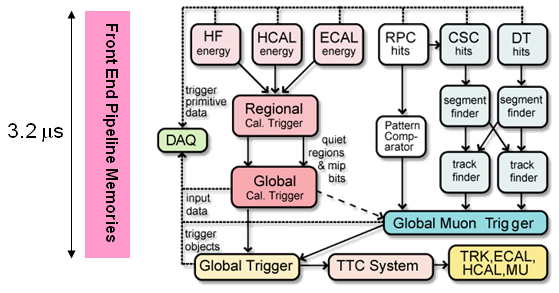
\includegraphics[width=\textwidth]{generated/LoneTrigger/level1trigger.pdf}
  \caption{The CMS \Lone Trigger system}
  \label{fig:figures_LoneTrigger_level1trigger}
\end{figure}

The CMS \Lone trigger system\cite{l1} is a pipelined dead-timeless system based 
on custom-built electronics.
The \Lone trigger is a combination of several sub systems, which are 
interconnected as depicted in 
Figure~\ref{fig:figures_LoneTrigger_level1trigger}.

Corse grain information from the electro-magnetic, hadronic and forward 
calorimeters is processed by the Regional Calorimeter Trigger (RCT), this is 
then passed to the Global Calorimeter Trigger (GCT) where the corse grain 
information is clustered in to physics objects, these objects are then passed 
to the Global Trigger where the \Lone accept decision is made. Due to the 
limited size of the pipe line this \Lone accept must be issued within 4.0 
$\mu$s.

The objects passed from the GCT to the GT include electro-magnetic objects, 
both electrons and photons as due to the lack of
tracking information at the \Lone trigger these objects are indistinguishable, 
jets and energy sums.

The RCT generates up to 72 isolated and non-isolated electro-magnetic objects, 
these are sorted by rank, which is equivalent to
transverse energy \ET. The four highest ranked electro-magnetic objects are 
then passed via the GCT to the GT at an equivalent data 
rate of 29 \Gbs per type.

Hadronic objects under go two clustering steps. First the transverse energy 
sums of the ECAL and corresponding HCAL towers are
calculated, the towers are then summed in to 4$\times$4 trigger regions, these 
are passed to the GCT at a data rate of 172.8 \Gbs.
These trigger regions are clustered in to jet candidates by the GCT and ranked. 
The jets are then sub-divided in the 
categories depending on their pseudo-rapidity and the result of $\tau$ 
identification. 

Energy sums come in two forms, the total transverse energy \ET which is the 
scalar sum of all transverse energies and the total 
jet transverse energy \HT which is calculated as the scalar sum of all jets 
above some programable threshold.

The missing energy equivalents of these \MET and \MHT are formed from the 
negative vector sum of the objects considered for the
transverse sums.



\section{Leve-1 Trigger Jet Algorithm} % (fold)
\label{sec:leve_1_trigger_jet_algorithm}

\textbf{FIXME: This is taken pretty much straight from \cite{gctcomm} might 
want to steal less??} 

The CMS detector can be un-rolled in the $\phi$ direction to form a rectangular 
grid of the 396 calorimeter regions, connected along the $\phi$ edge. The
rectangle 18 $\phi$ divisions (from $-180^{\circ} < \phi \leq 180^{\circ}$) by 
22 $\eta$ divisions ( from $-5 < \eta < 5$). Each $\phi$ division corresponds 
to 20$^{\circ}$. The $\eta$ divisions correspond to $\Delta\eta$ $= 0.5$ in the 
forward calorimeters and to $\Delta\eta \approx 0.348$ in the barrel.
A pictorial representation of this can be seen in 
figure~\ref{fig:figures_LoneTrigger_jetfindermappings}.

\begin{figure}[ht]
  \centering
    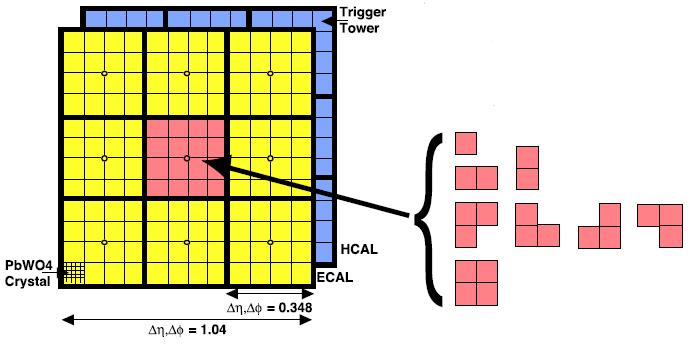
\includegraphics[width=\textwidth]{figures/LoneTrigger/level1jetalgo.jpg}
  \caption{The 3 $\times$ 3 jet-finder window at \Lone. Each cell represents a 
  trigger tower, which is the sum of the HCAL and ECAL transverse energies. The 
  $\tau$-jet veto patterns are shown to the right.}
  \label{fig:figures_LoneTrigger_level1jetalgo}
\end{figure}


A jet candidate is created if the sum of the ECAL and HCAL energies of the 
central calorimeter region has an energy deposit larger than all of its 
neighbours, as shown in figure~\ref{fig:figures_LoneTrigger_level1jetalgo}
The jet is centered at this region where $p_{T}^{central} > p_{T}^{surrounding}$
and the transverse energies of the surrounding regions are summed in to the 
central region. The jet is then classified as a $\tau$ jet if \mETA $< 3.0$ and 
none of the $\tau$ veto bits are set. If any $\tau$ vetoes are set the jet is 
classified as a central jet. The jet is classified as forward if $ 3.0 < \mETA 
< 5.0$

The $\tau$-vetoes are set by the RCT depending on whether or not the energy 
depositions in up to four contiguous trigger towers are below a programmable 
fraction of the regional \ET as shown in 
Figure~\ref{fig:figures_LoneTrigger_level1jetalgo}.

It is possible to apply separate jet energy corrections to each of the sub 
categories of GCT jets. These corrections are discussed in detail in 
Section~\ref{sec:lone_trigger_performance}

\begin{figure}[ht]
  \centering    
  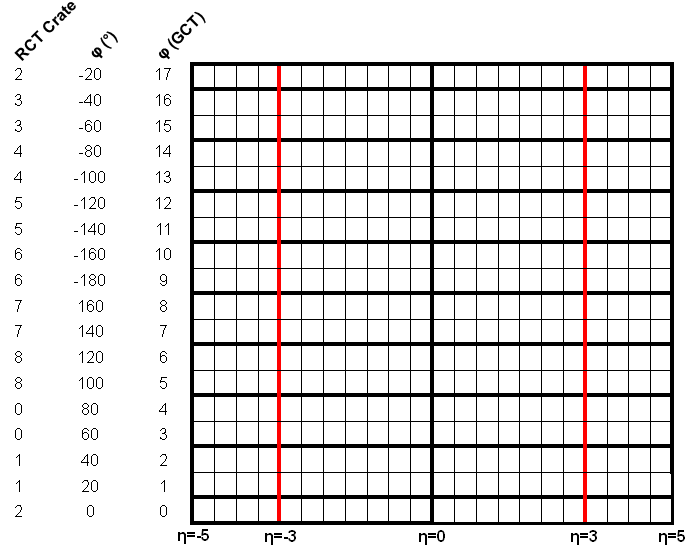
\includegraphics[width=\textwidth]{figures/LoneTrigger/jetfindermappings.png}
  \caption{caption}
  \label{fig:figures_LoneTrigger_jetfindermappings}
\end{figure}

In order to reduce the total data duplicated and shared between the jet finders
the GCT employs a pre-clustering algorithm, which involves 18 jet finders 
operating simultaneously over the whole detector. These jet finders then only
share information with neighboring regions when the clustered jets are found.
Figure~\ref{fig:figures_LoneTrigger_jetfindermappings} shows the boundaries 
between which the jet finders operate, these map naturally on to one RCT crate 
per jet finder. A maximum of 3 jets can be found on each of the $\phi$ strips
acted on by the jet finders, this gives a maximum of 108 jets per event. In
order to preserve continuity across the $\eta = 0$ boundary, the two adjacent
trigger regions are shared between the jet finders.


\begin{figure}[ht]
  \centering
 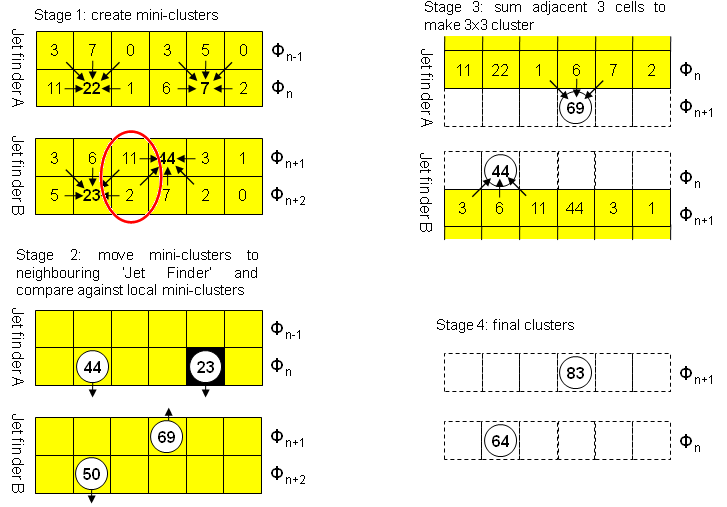
\includegraphics[width=\textwidth]{figures/LoneTrigger/jetfinderfunction.png}
  \caption{caption}
  \label{fig:figures_LoneTrigger_jetfinderfunction}
\end{figure}


An example of the jet finding is shown in
Figure~\ref{fig:figures_LoneTrigger_jetfinderfunction}. The first step is to 
create a $2 \times 3$ mini cluster around any local maxima found in the $12 
\times 2$ strip. Equality statements are imposed so that the central cell is 
greater than its neighbors in some directions and greater than or equal to the 
neighbors other directions to enforce a gap of at least one trigger region in 
both $\eta$ and $\phi$ between the centers of the clustered jets.

In the second step the jet finder transfers the three largest mini clusters on 
a given $\phi$ strip to the closest $\phi$ strip on the neighboring jet finder.
These are then compared against the existing mini clusters in that $\phi$ strip,
those that are adjacent or diagonally agecent to a larger mini cluster are 
removed. The inequalities statements are then reimposed to prevent problems
with clusters having the same energies. In the final stages the mini clusters
have their three adjacent regions summed in to produce a $3 \times 3$ jet
cluster. Finally the four highest ranked jets are corrected and passed to the 
GT.
% section leve_1_trigger_jet_algorithm (end)




\section{\Lone Trigger Performance} % (fold)
\label{sec:lone_trigger_performance}
\textbf{FIXME: Can i just copy the stuff out of the L1 performance note here 
for the corrections? I will need to re-make a bunch of the plots though :( Jobs 
set running as of 24th july.}
% section lone_trigger_performance (end)

\section{\Lone Trigger Pile-up Mitigation} % (fold)
\label{sub:lone_trigger_pile_up_mitigation}
Due to the lack of a requirement of a jet seed threshold, soft non-collimated 
jets, such as those expected in a high pile up environment are found. Trigger 
decisions are then made using these pile up jets.

This is less of a problem for the single jet triggers which have a high $P_{T}$ 
threshold. However the \HT triggers, where \HT = $\sum_{jets}E_{T}^{jet}$ and 
the requirement of \ET$^{jet} \geq $10 \GeV is made, see a large increase in 
rate due to pile-up, this is due to the low energy  threshold required for a 
jet to be added to the \HT sum.

To counteract the effect of pile up on trigger rate we study the effects of 
requiring a jet seed threshold on the rate and efficiency of the individual jet 
and \HT triggers.

Figure~\ref{fig:figures_LoneTrigger_level1jetalgo} depicts 3$\times$3 trigger
regions, each of which are built from 4$\times$4 trigger towers. In this case 
the central region is the jet seed. The proposed change would require there to 
be a threshold energy in the seed region.

The study of using jet seed thresholds of 2 and 5 \GeV is presented. The 
maximum energy of effected jets is 18 \GeV when requiring a seed of 2 \GeV and 
45 \GeV when requiring a seed of 5 \GeV for jets made from $3\times3$ trigger 
regions. The jet clustering is performed before the \Lone jets are corrected 
according to their \ET and $\eta$, hence the effects are manifested in trigger 
decisions for \Lone jets above 18 or 45 \GeV.



\begin{figure}[h!]
    \centering
    \subfigure[GCT internal uncorrected jet \ET distributions for the same 
    events with a 0, 2 or 5 \GeV seed requirement.]{
          \label{fig:GCTrankRAW}
          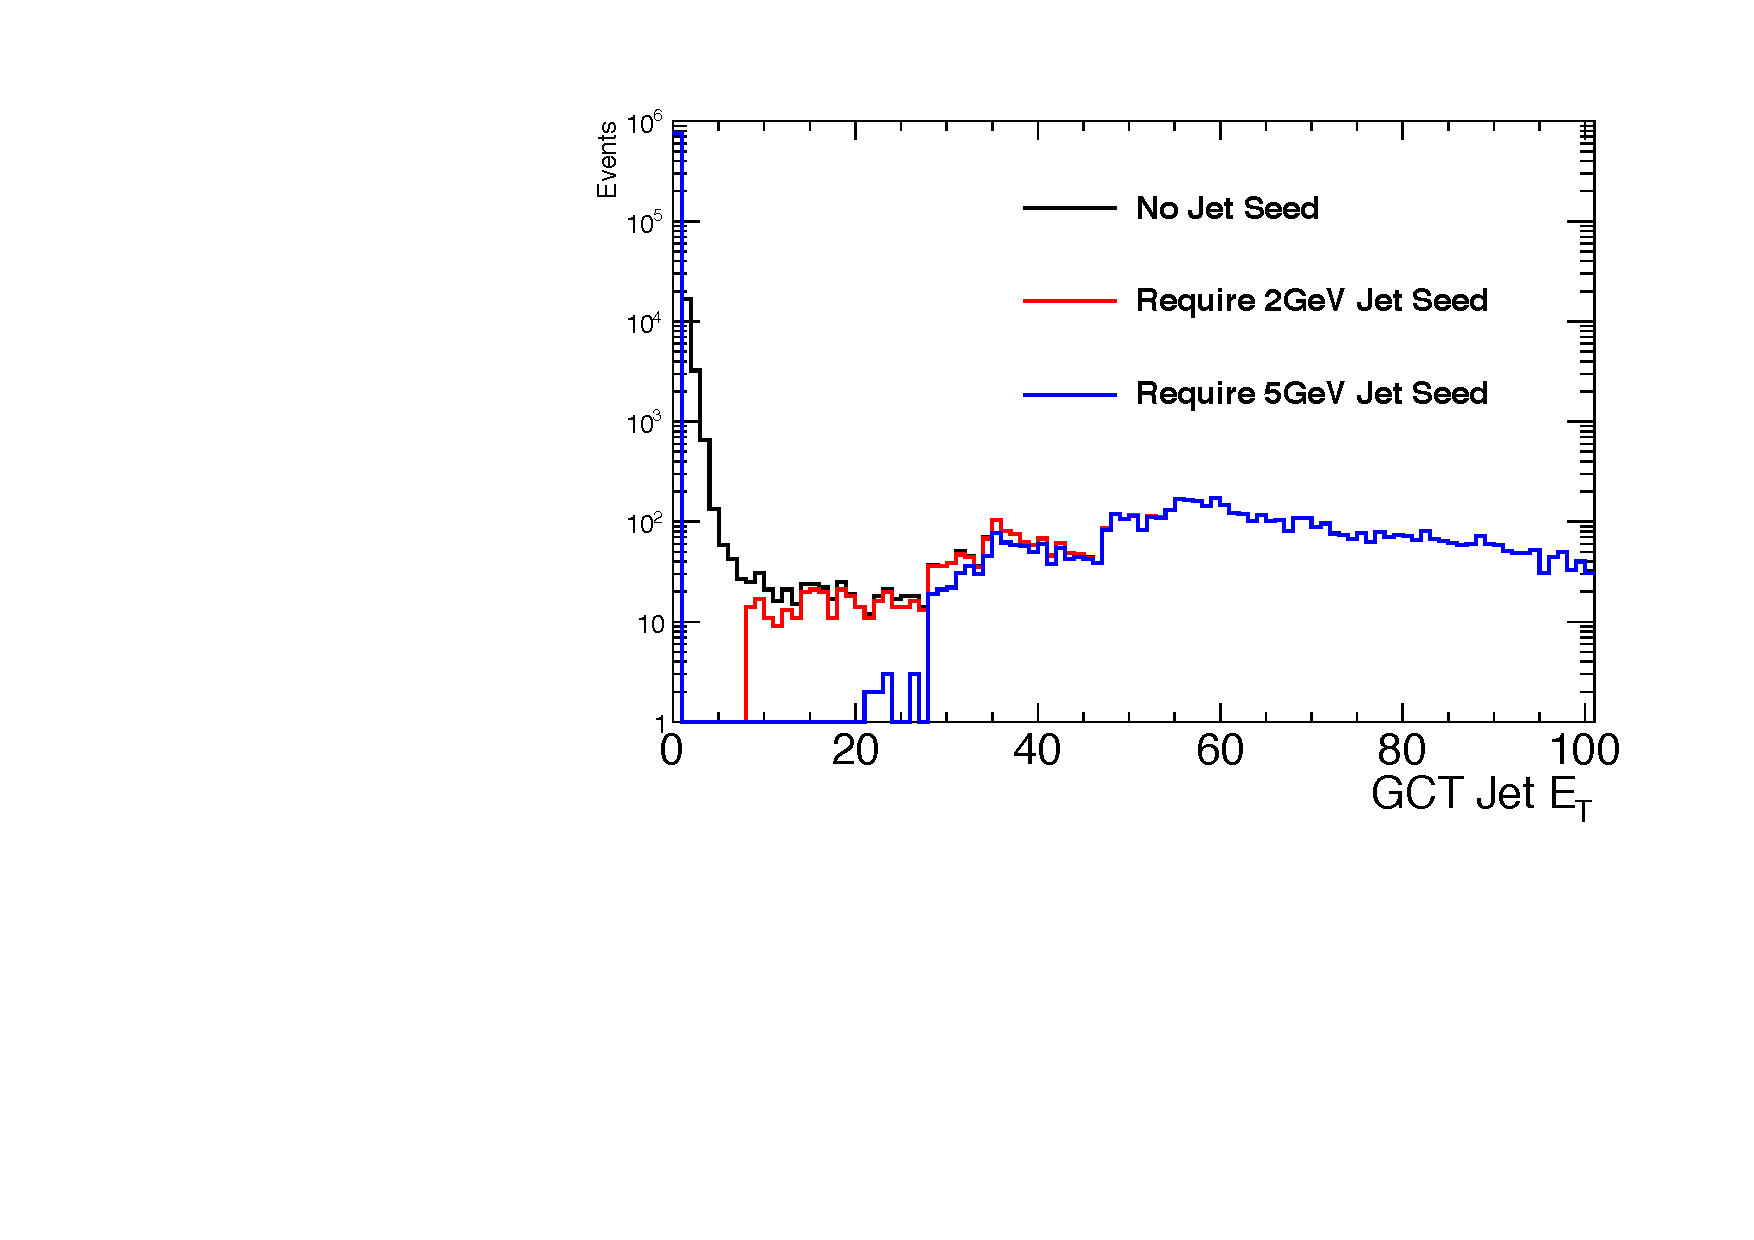
\includegraphics[width=0.45\textwidth]{generated/LoneTrigger/GCT_Jet_Rank_highPU.pdf}
     }
    \subfigure[Efficiency of applying a requirement of 2 or 5 \GeV with respect 
    to no requirement.]{
          \label{fig:GCTrankRatio}
          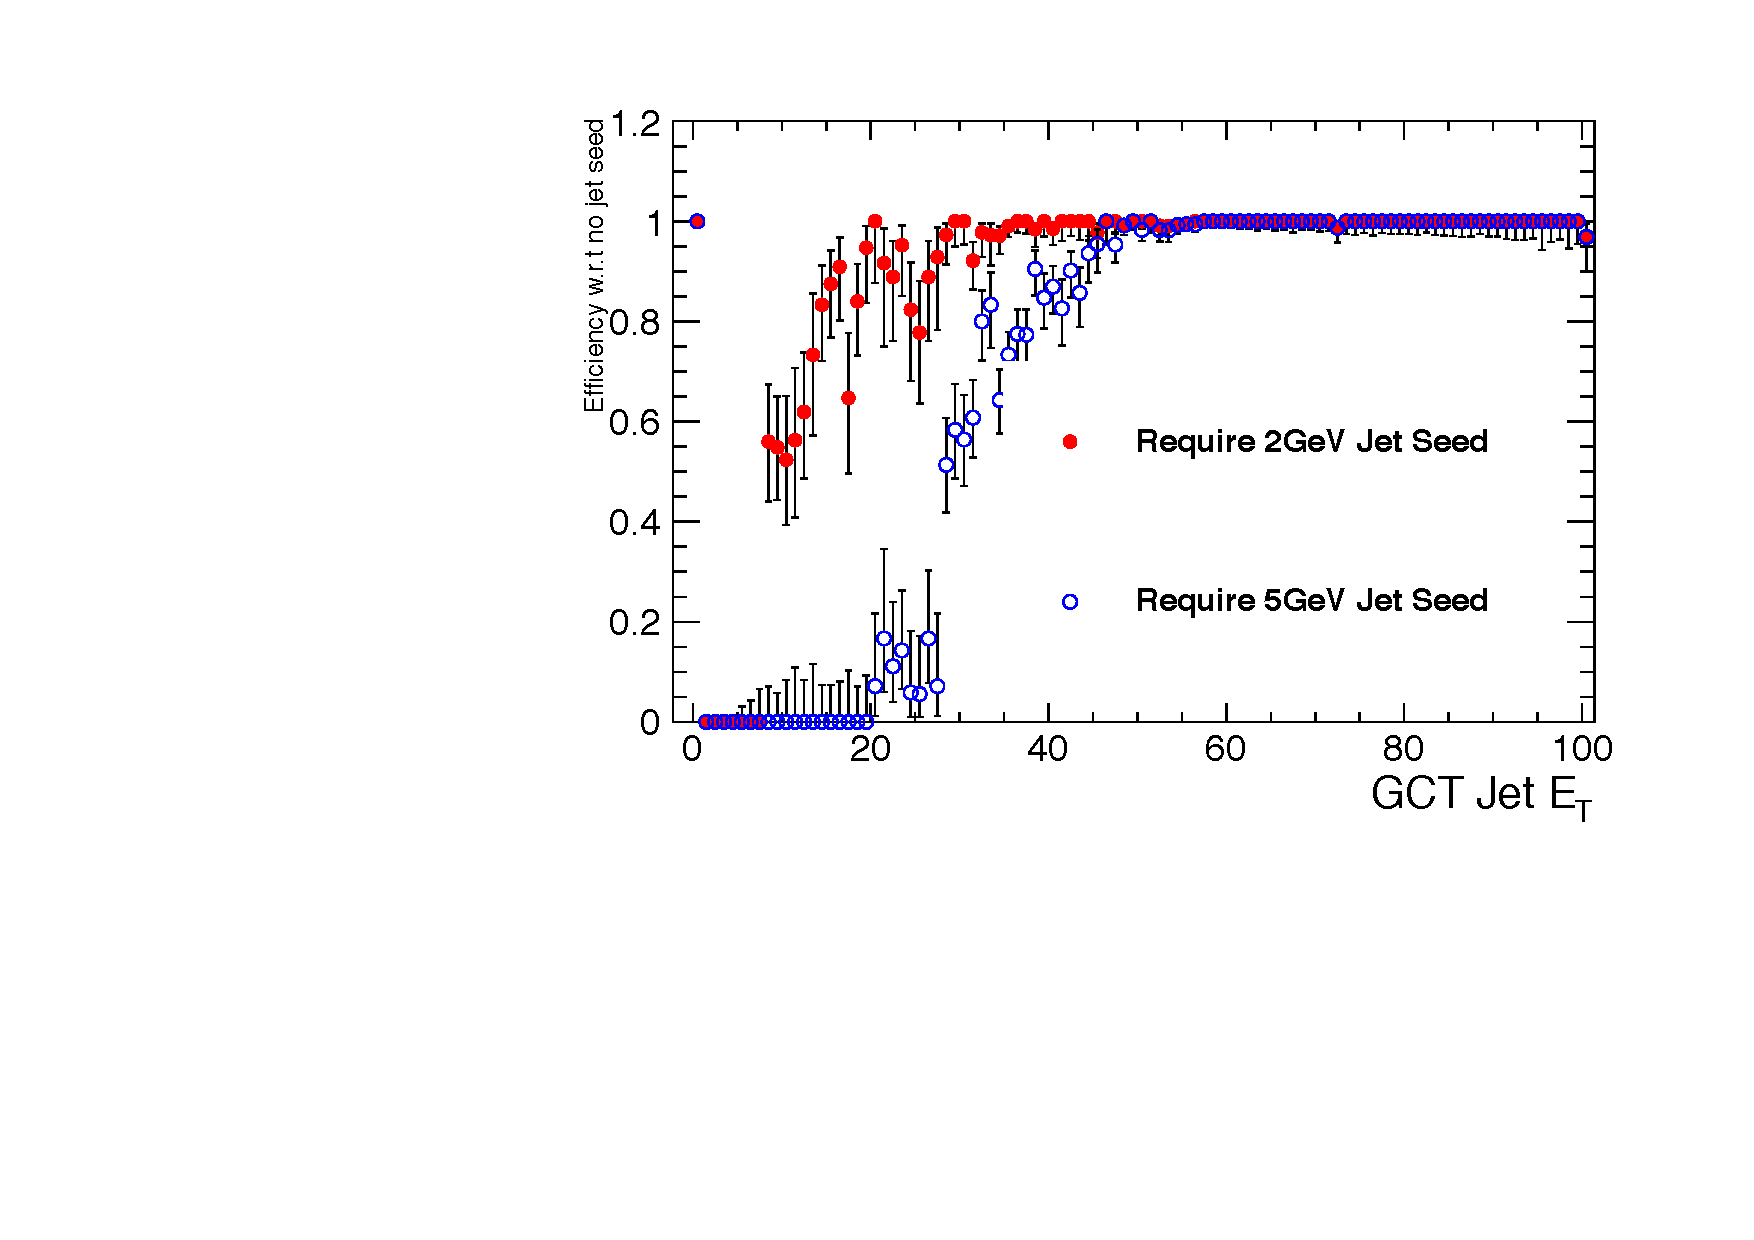
\includegraphics[width=0.45\textwidth]{generated/LoneTrigger/GCT_Jet_Rank_highPU_ratio.pdf}
     }
    \caption{Effect of requiring a jet seed threshold on GCT internal jets.}
    \label{fig:GCTrank}
\end{figure}


Figure~\ref{fig:GCTrank} shows how the different threshold requirements effect 
the rank of the internal GCT jets. The effect is to remove all jets below 
2(5)\GeV and to cut out jets from the low end of the distribution. From 
Figure~\ref{fig:GCTrankRatio} it is possible to see the point beyond which the 
requirement of a jet seed has no effect. For a cut of 2 \GeV jets above an 
uncorrected \ET of $\approx$ 35 \GeV are not effected, for a seed threshold of 
5 \GeV jets above an uncorrected \ET 55 \GeV are not effected.


\subsection{Effect on trigger rates} % (fold)
\label{sec:Effects on Rate}
The effects of applying a seed threshold are quantified in terms of the level of rate
reduction in the \Lone hadronic triggers.
Three triggers are studied, they are:
\begin{itemize}
  \item L1$\_$SingleJet50 - Level one trigger requring at least one jet with a 
  corrected \ET $\geq$ 50 \GeV.
  \item L1$\_$HTT100 - Level one trigger requring \HT $\geq 100$ \GeV.
  \item L1$\_$QuadJet38 - Level one trigger requring at least four jets in the 
  event with \ET $\geq$ 38 \GeV.

\end{itemize}
\subsection{Low Pile Up} % (fold)
\label{sub:Low Pile Up}
A small effect on trigger rates in the low pile up scenario is expected due to 
the majority of energy deposited in the calorimeters coming from hard 
scattering.
\begin{figure}[h!]
    \centering
    \subfigure[]{
          \label{fig:HTLowPU}
          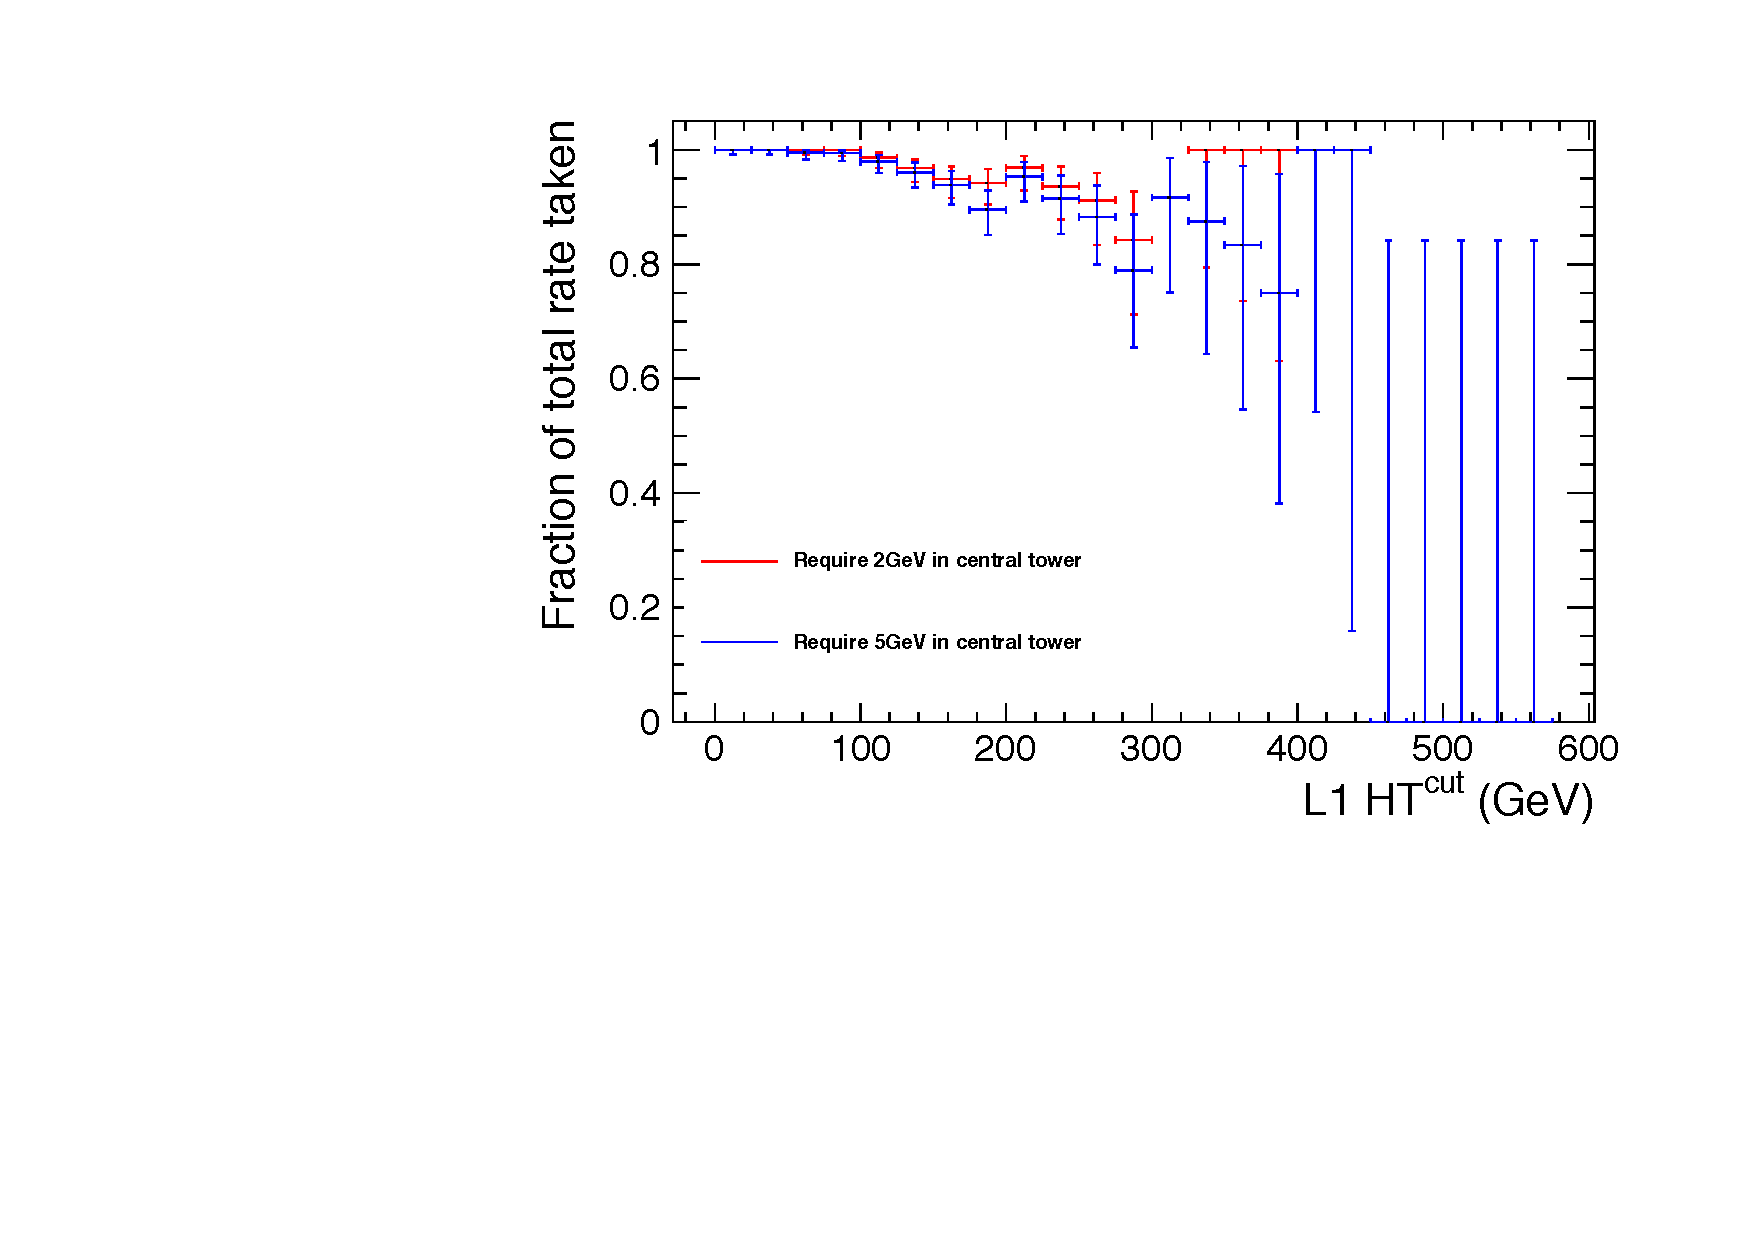
\includegraphics[width=0.46\textwidth]{figures/LoneTrigger/HT_LowPU_RateReduction.pdf}
     }
    \subfigure[]{
          \label{fig:cenJetLowPU}
          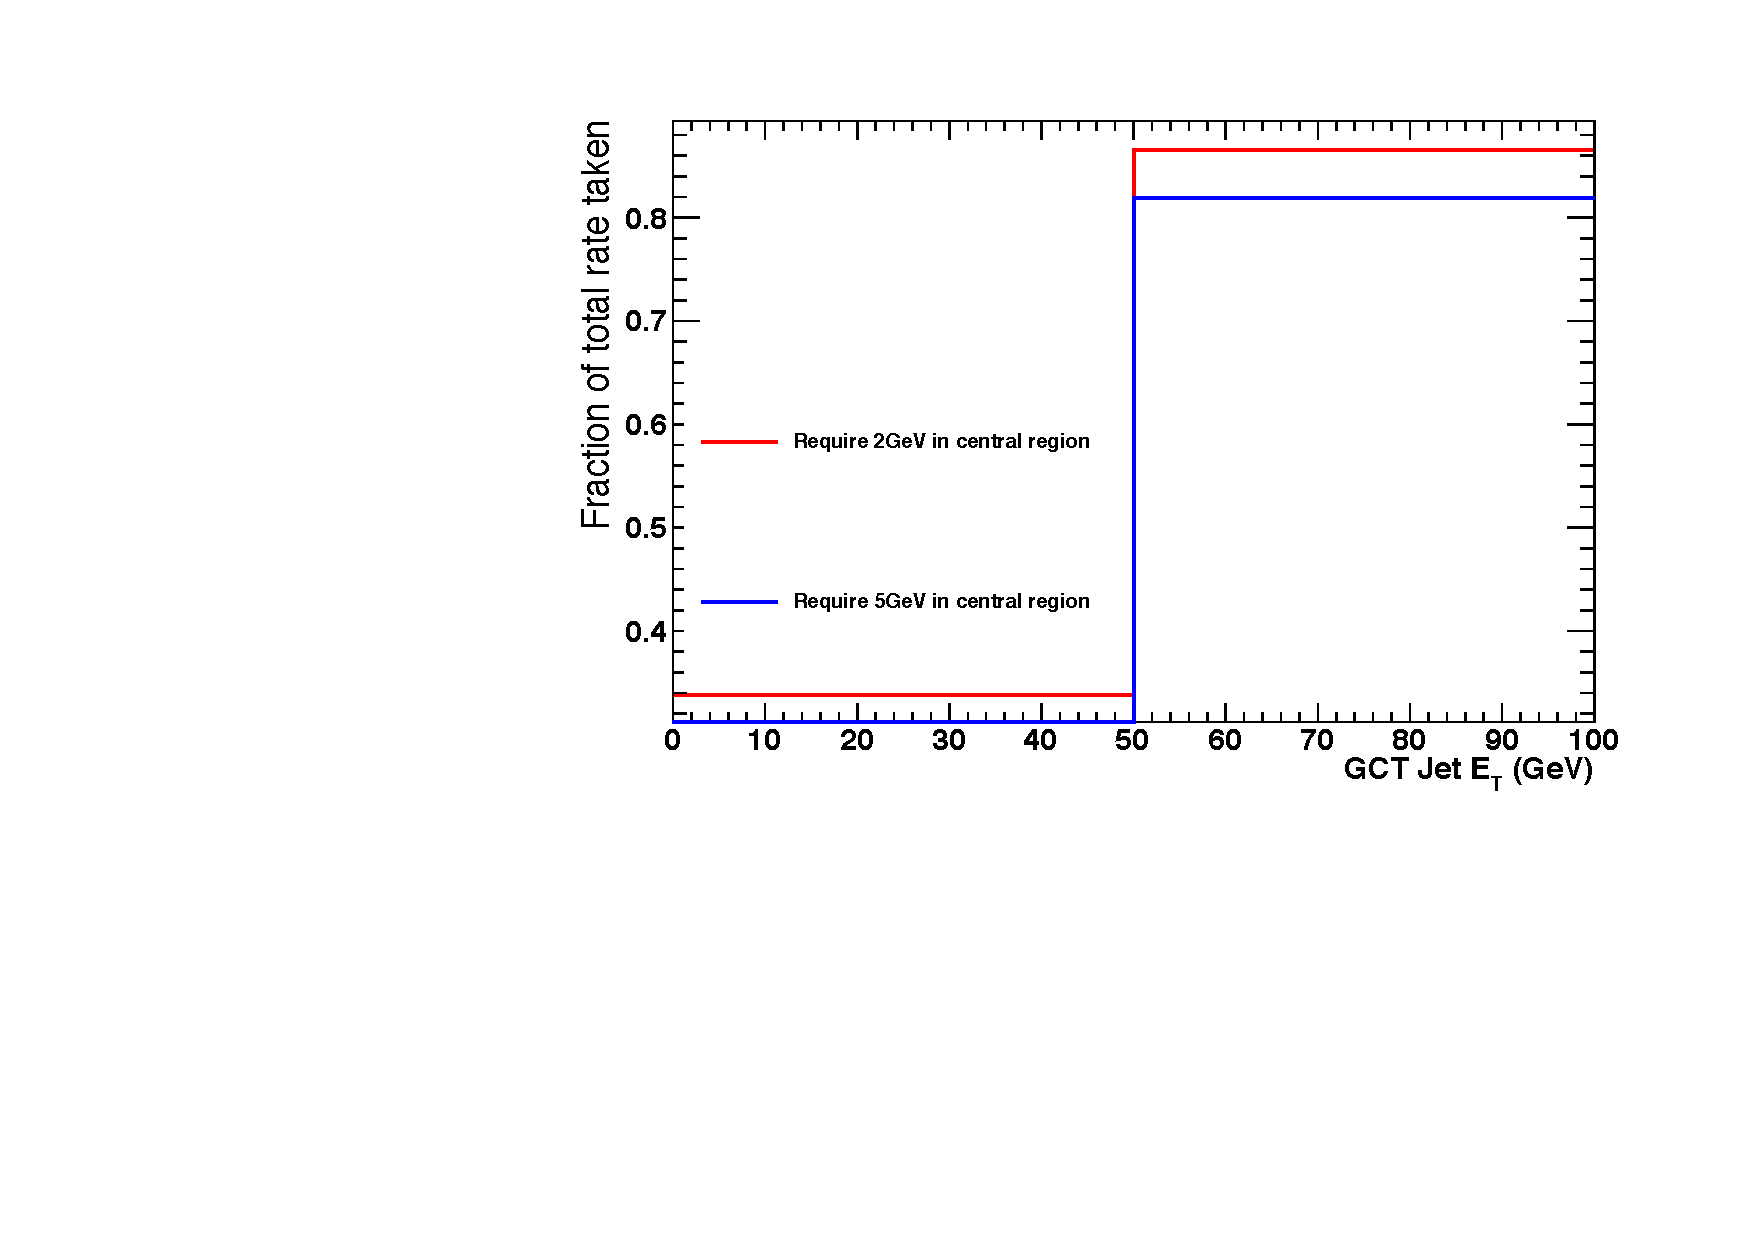
\includegraphics[width=0.46\textwidth]{figures/LoneTrigger/Cen_Tau_LowPU_RateReduction.pdf}
     }
     \newline
    \subfigure[]{
          \label{fig:quadJetLowPU}
          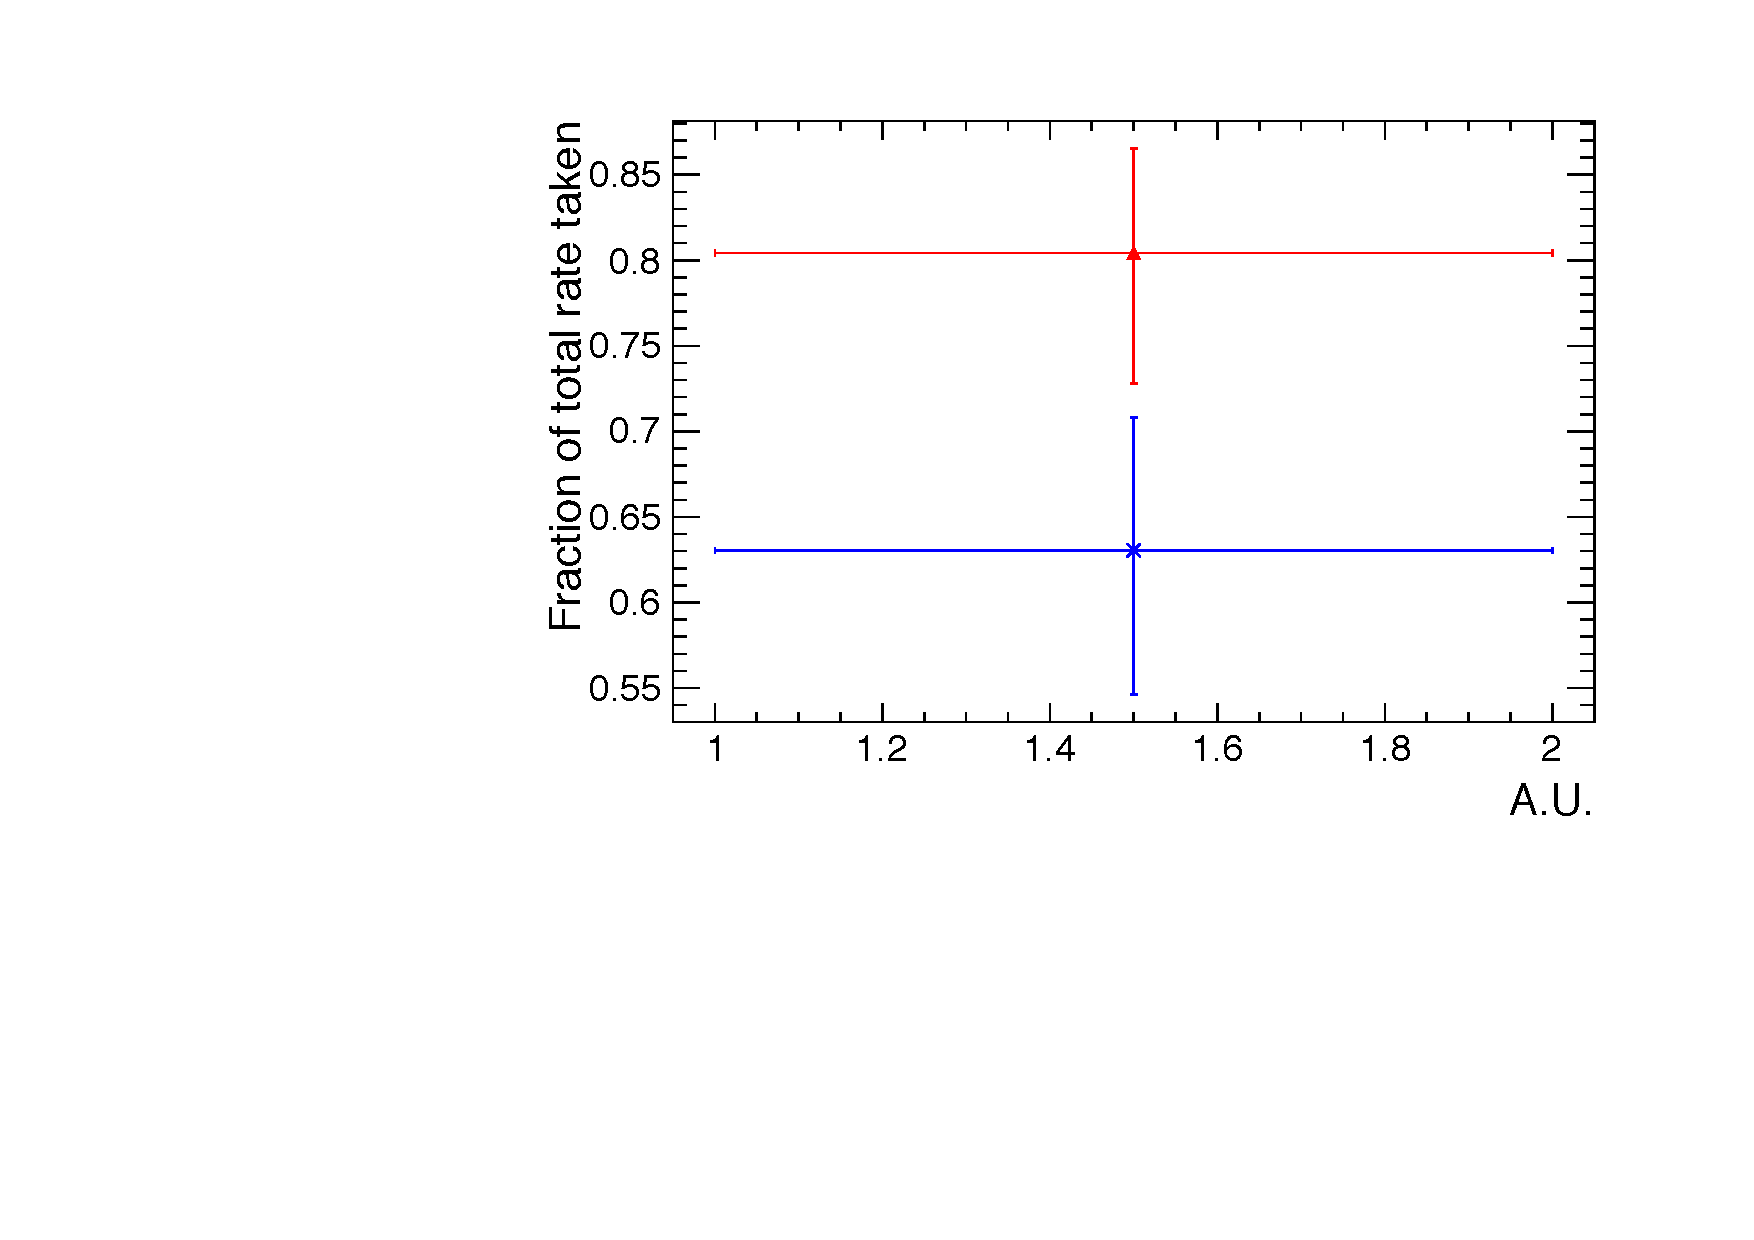
\includegraphics[width=0.46\textwidth]{figures/LoneTrigger/QuadJet_38Cen_LowPU_RateReduction.pdf}
     }
    \caption{Rate reductions for various \Lone algorithms when applying a 2,5 \GeV seed tower requirement, in low pile up
     conditions. Figure (a) shows the rate reduction for \HT triggers at low pile up in cut steps of 25 \GeV. Figure (b) shows the 
     rate reduction for jets with in $|\eta| <3.$ and $\pt > 50$ \GeV. Figure (c) shows the rate reduction for a quad jet trigger,
     with jet $|\eta| <3.$ and $\pt > 38$ \GeV.}
    
    \label{fig:lowpuratereduction}
\end{figure}

\begin{table}
\caption{Summary of rate reduction during low pile up conditions.}
\begin{tabular}{c|c|c}

\hline
Trigger & $\%$ of rate taken with 2\GeV requirement & $\%$ of rate taken with 5\GeV requirement\\
\hline
L1$\_$HTT100 & $98.6 \pm 11.6\%$ & $97.9 \pm 11.6\%$\\
\hline
L1$\_$QuadJet38 & $100.0 \pm 0.0\%$ & $85.3 + 6.2 - 8.7\%$\\
\hline
L1$\_$Jet50 & $100.0 + 0.0 - 12.3\%$ & $85.7 + 9.1 - 15.8\%$\\
\hline
\end{tabular}
\label{tab:lowpuratereduction}


\end{table}

Table~\ref{tab:lowpuratereduction} shows the rate reduction of requiring a 2 or 
5 \GeV seed threshold with respect to requiring no seed threshold.

% subsection Low Pile Up (end)

\subsection{High Pile Up} % (fold)
\label{sub:High Pile Up}
Pile up is expected to add a small quantity of energy to the entire calorimeter 
system, this energy comes in the form of soft non-collimated jets. These 
objects are then not reconstructed if the topological cut of applying a seed
threshold is required.

\begin{figure}[h!]
    \centering
    \subfigure[]{
          \label{fig:HTHighPU}
          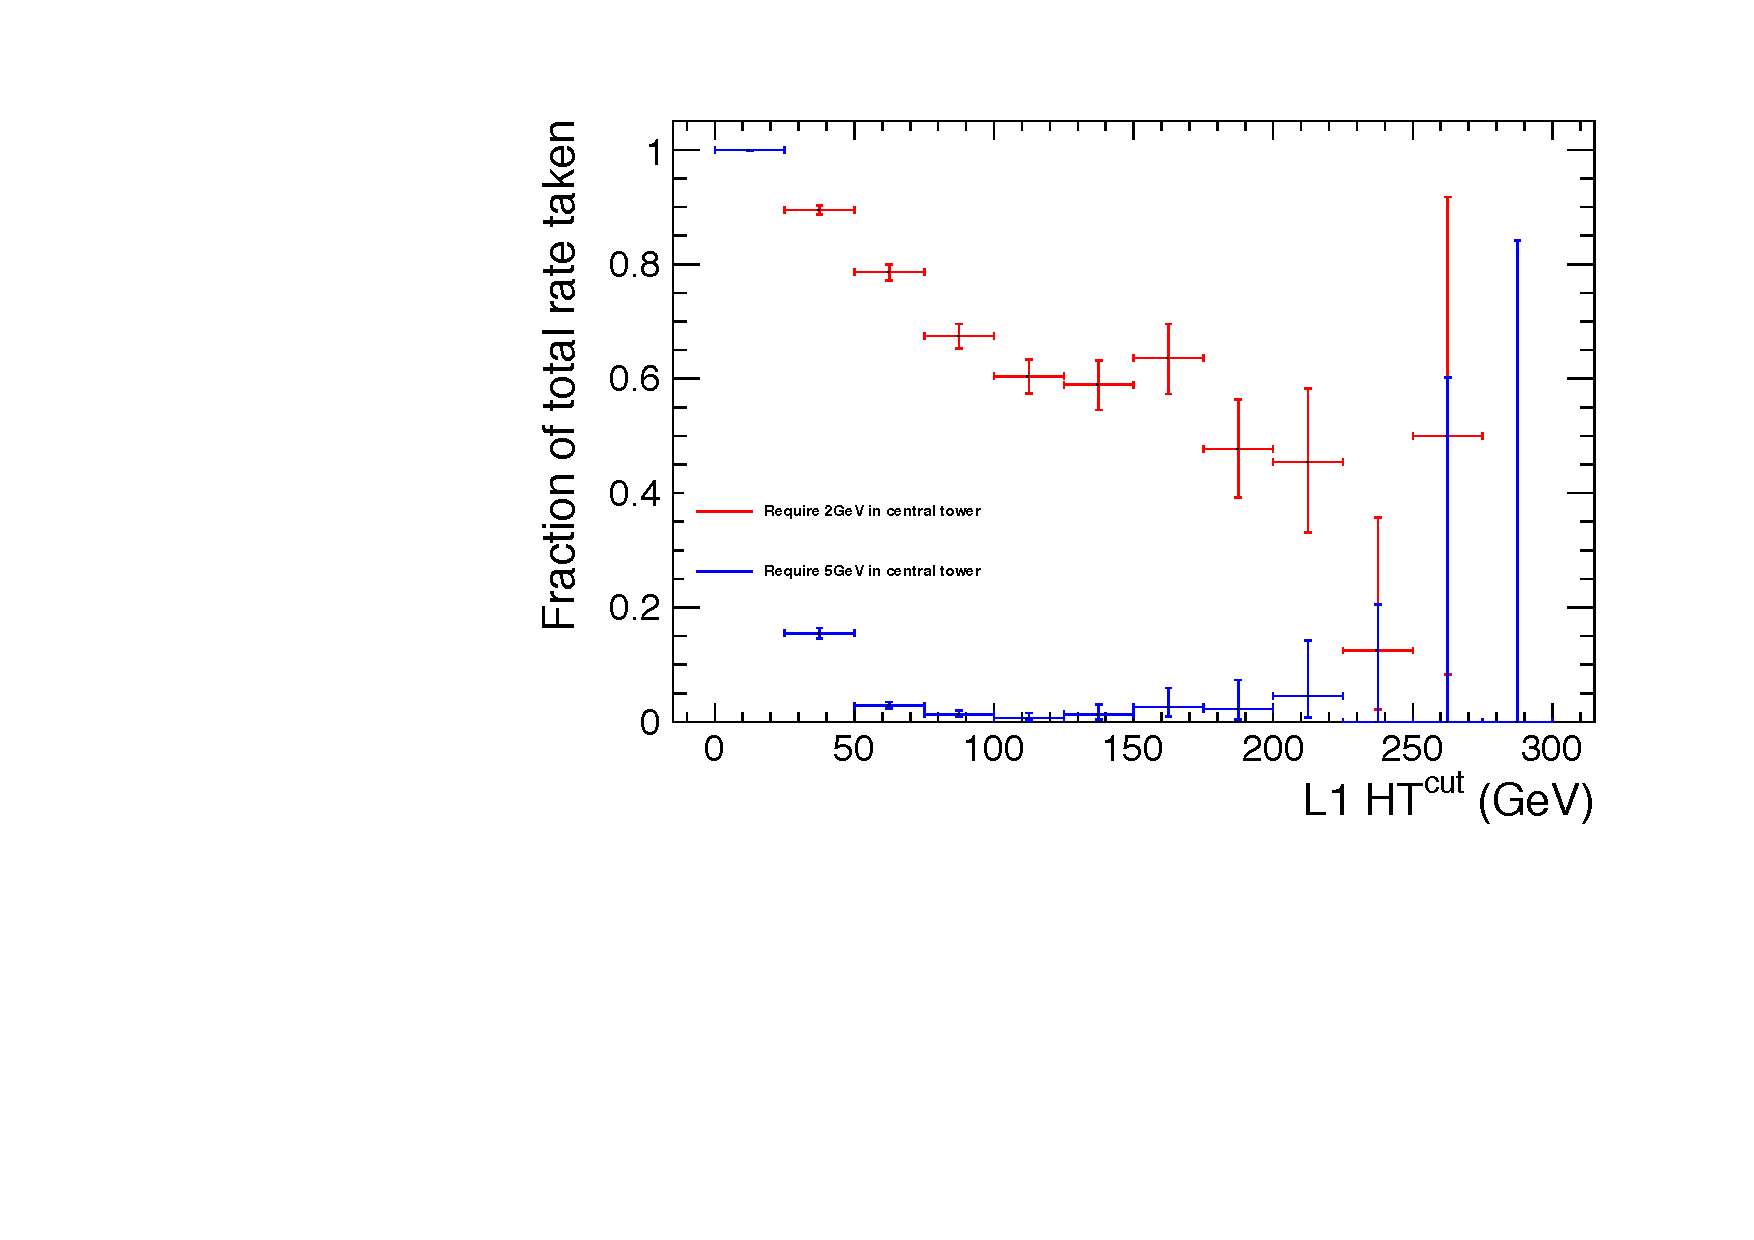
\includegraphics[width=0.46\textwidth]{figures/LoneTrigger/HT_HighPU_RateReduction.pdf}
     }
    \subfigure[]{
          \label{fig:cenJetHighPU}
          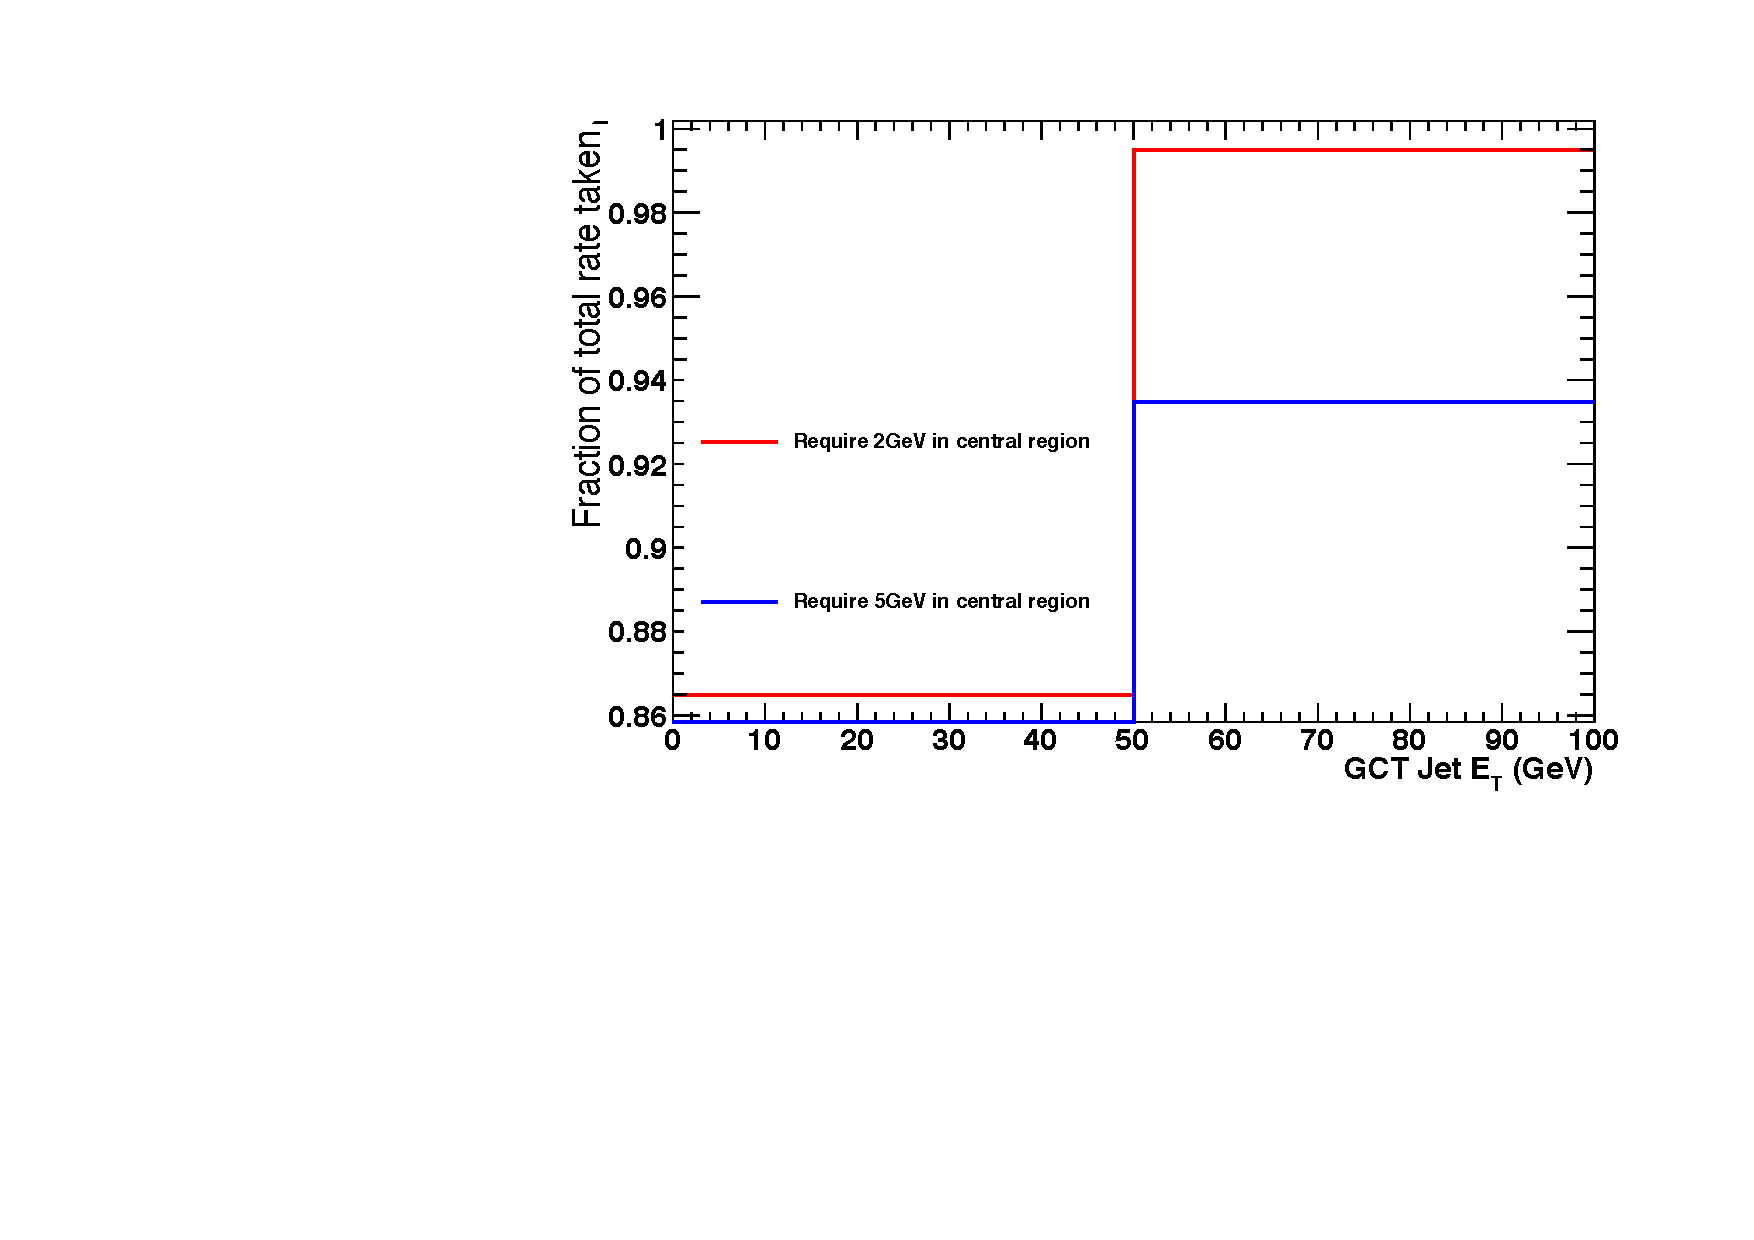
\includegraphics[width=0.46\textwidth]{figures/LoneTrigger/Cen_Tau_HighPU_RateReduction.pdf}
     }
     \newline
    \subfigure[]{
          \label{fig:quadJetHighPU}
          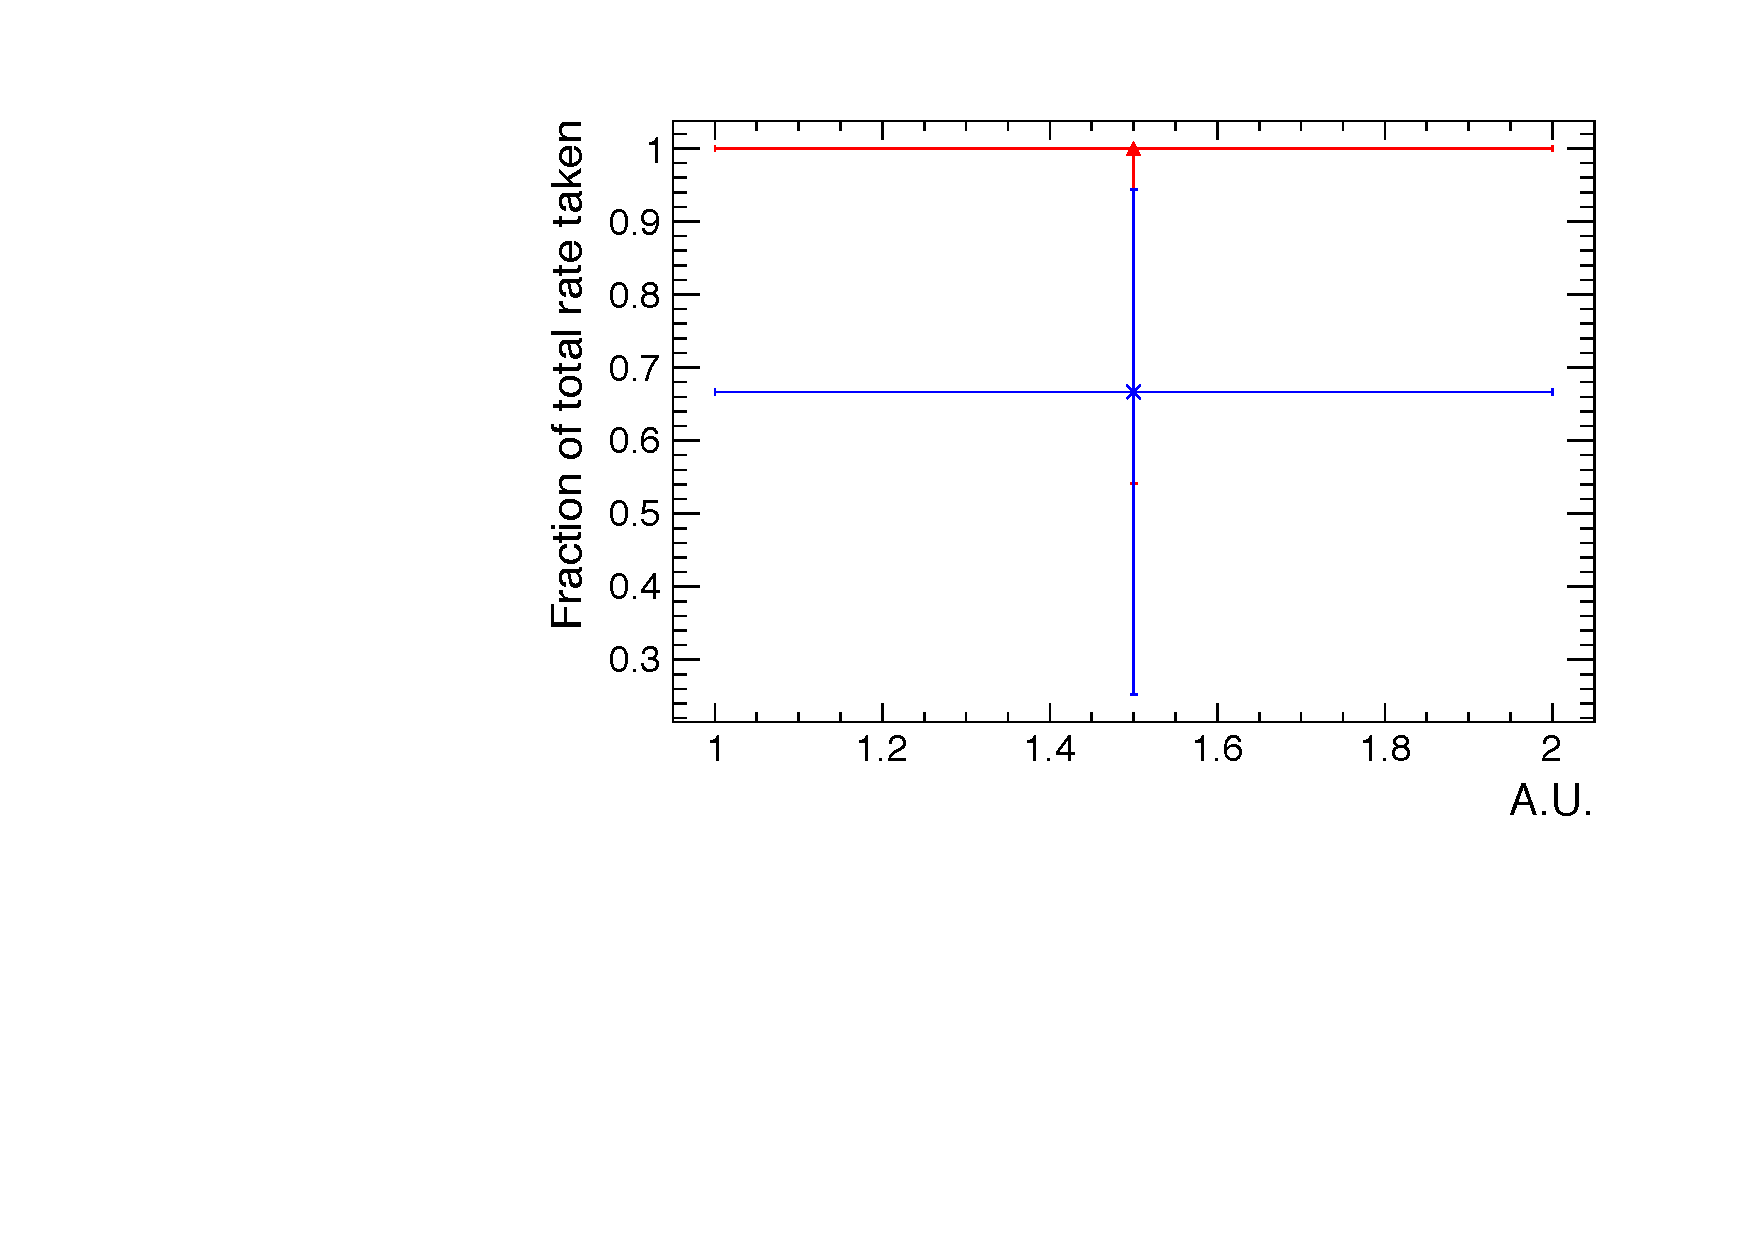
\includegraphics[width=0.46\textwidth]{figures/LoneTrigger/QuadJet_38Cen_HighPU_RateReduction.pdf}
     }
    \caption{Rate reductions for various \Lone algorithms when applying a 2,5 
    \GeV seed tower requirement, in high pile up
    conditions. Figure (a) shows the rate reduction for \HT triggers at high 
    pile up, in cut steps of 25 \GeV. Figure (b) shows
    the rate reduction for jets with in $|\eta| <3.$ and $\pt > 50$\GeV. Figure 
    (c) shows the rate reduction for a quad jet
    trigger, with jet $|\eta| <3.$ and $\pt > 38$\GeV}
    
    \label{fig:highpuratereduction}
\end{figure}

\begin{table}
\caption{Summary of rate reduction during high pile up conditions.}
  
\begin{tabular}{c|c|c}
\hline
Trigger & $\%$ of rate taken with 2\GeV requirement & $\%$ of rate taken with 5\GeV requirement\\
\hline
L1$\_$HTT100 & $60.4 \pm 5.7\%$ & $0.67 +/- 0.67\%$\\
\hline
L1$\_$QuadJet38 & $71.4 + 18.2 - 25.9\%$ & $57.1 + 22.3 - 24.8\%$\\
\hline
L1$\_$Jet50 & $100.0 + 0.0 - 7.7\%$ & $73.9 + 9.8 - 12.3\%$\\
\hline

\end{tabular}
\label{tab:highpuratereduction}
\end{table}
Table~\ref{tab:highpuratereduction} shows the rate reduction of requiring a 2 
or 5 \GeV seed threshold with respect to requiring no seed threshold in high 
pile up conditions.


% subsection High Pile Up (end)

% section Effects on Rate (end)
\subsection{Effect on trigger efficiency} % (fold)
\label{sec:Effects of requiring a jet seed on offline efficiency}
Section~\ref{sec:Effects on Rate} shows that requiring a jet seed threshold
substantially reduces the trigger acceptance rate at in high pile up conditions.

However the aim of requiring a jet seed is to reduce rate, but not at the cost 
of physics. In this section we look at the effects of requiring a seed 
threshold, whilst requiring some loose, generic offline selection on the 
hadronic objects.

The change in efficiency is measured under low pile up conditions where the 
least extra energy added to the event. This gives a worse case estimate of the 
effect of requiring a jet seed on the offline efficiency.

Each offline reconstructed calorimeter jet must adhere to the following quality 
criteria:
\begin{itemize}
\item Pass loose calorimeter ID 
\item \PT $\geq$ 30 \GeV.
\item $|\eta| \leq$ 3.0.
\item Matched to a \Lone jet with $\Delta R \leq 0.5$.
\end{itemize}
Where loose calorimeter ID is defined as; Electro-Magnetic fraction $> 0.01$, fraction of energy in the Hybrid Photo Diodes $< 
0.98$ and the number of n90hits $> 1$.

\begin{figure}[h!]
    \centering
    \subfigure[]{
          \label{fig:HTlowPURECO}
          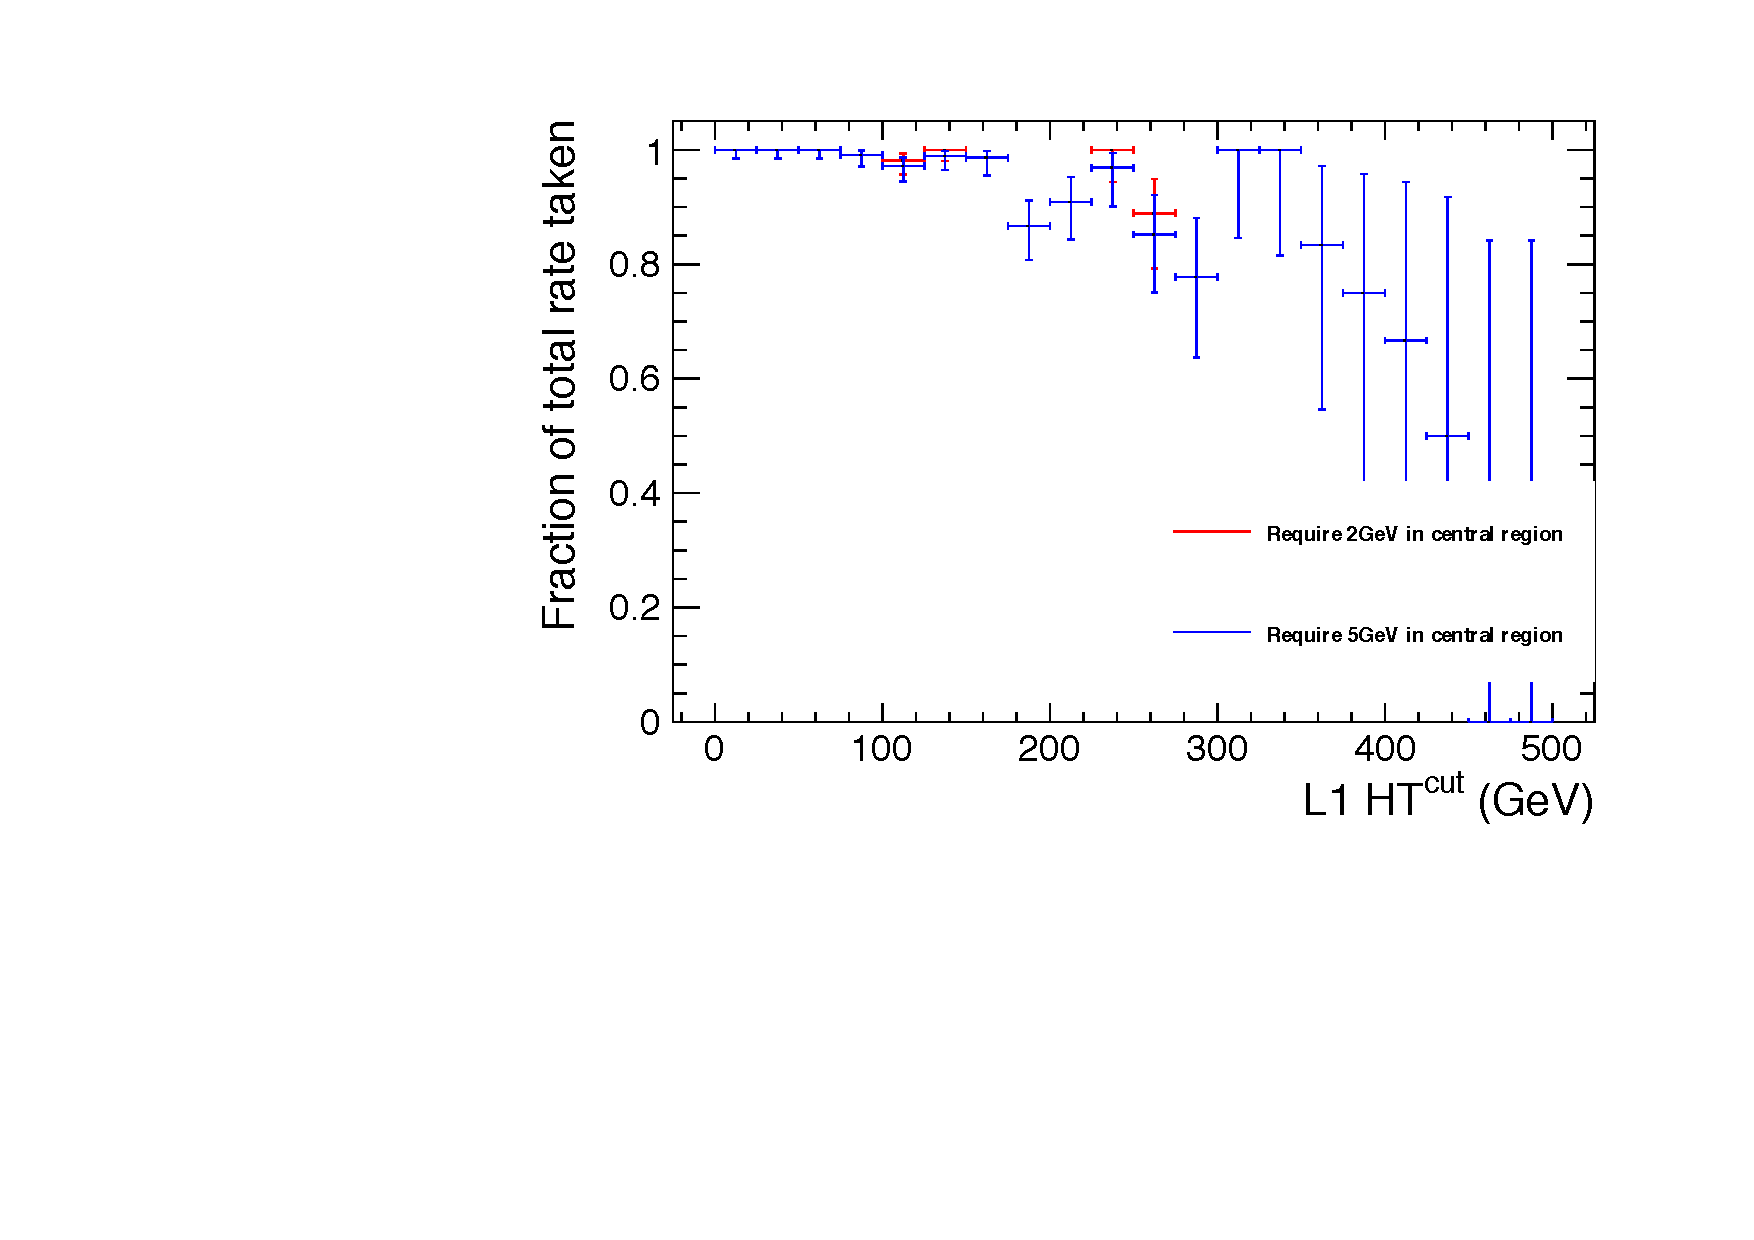
\includegraphics[width=0.46\textwidth]{figures/LoneTrigger/HT_LowPU_RECO.pdf}
     }
    \subfigure[]{
          \label{fig:cenJetLowPURECO}
          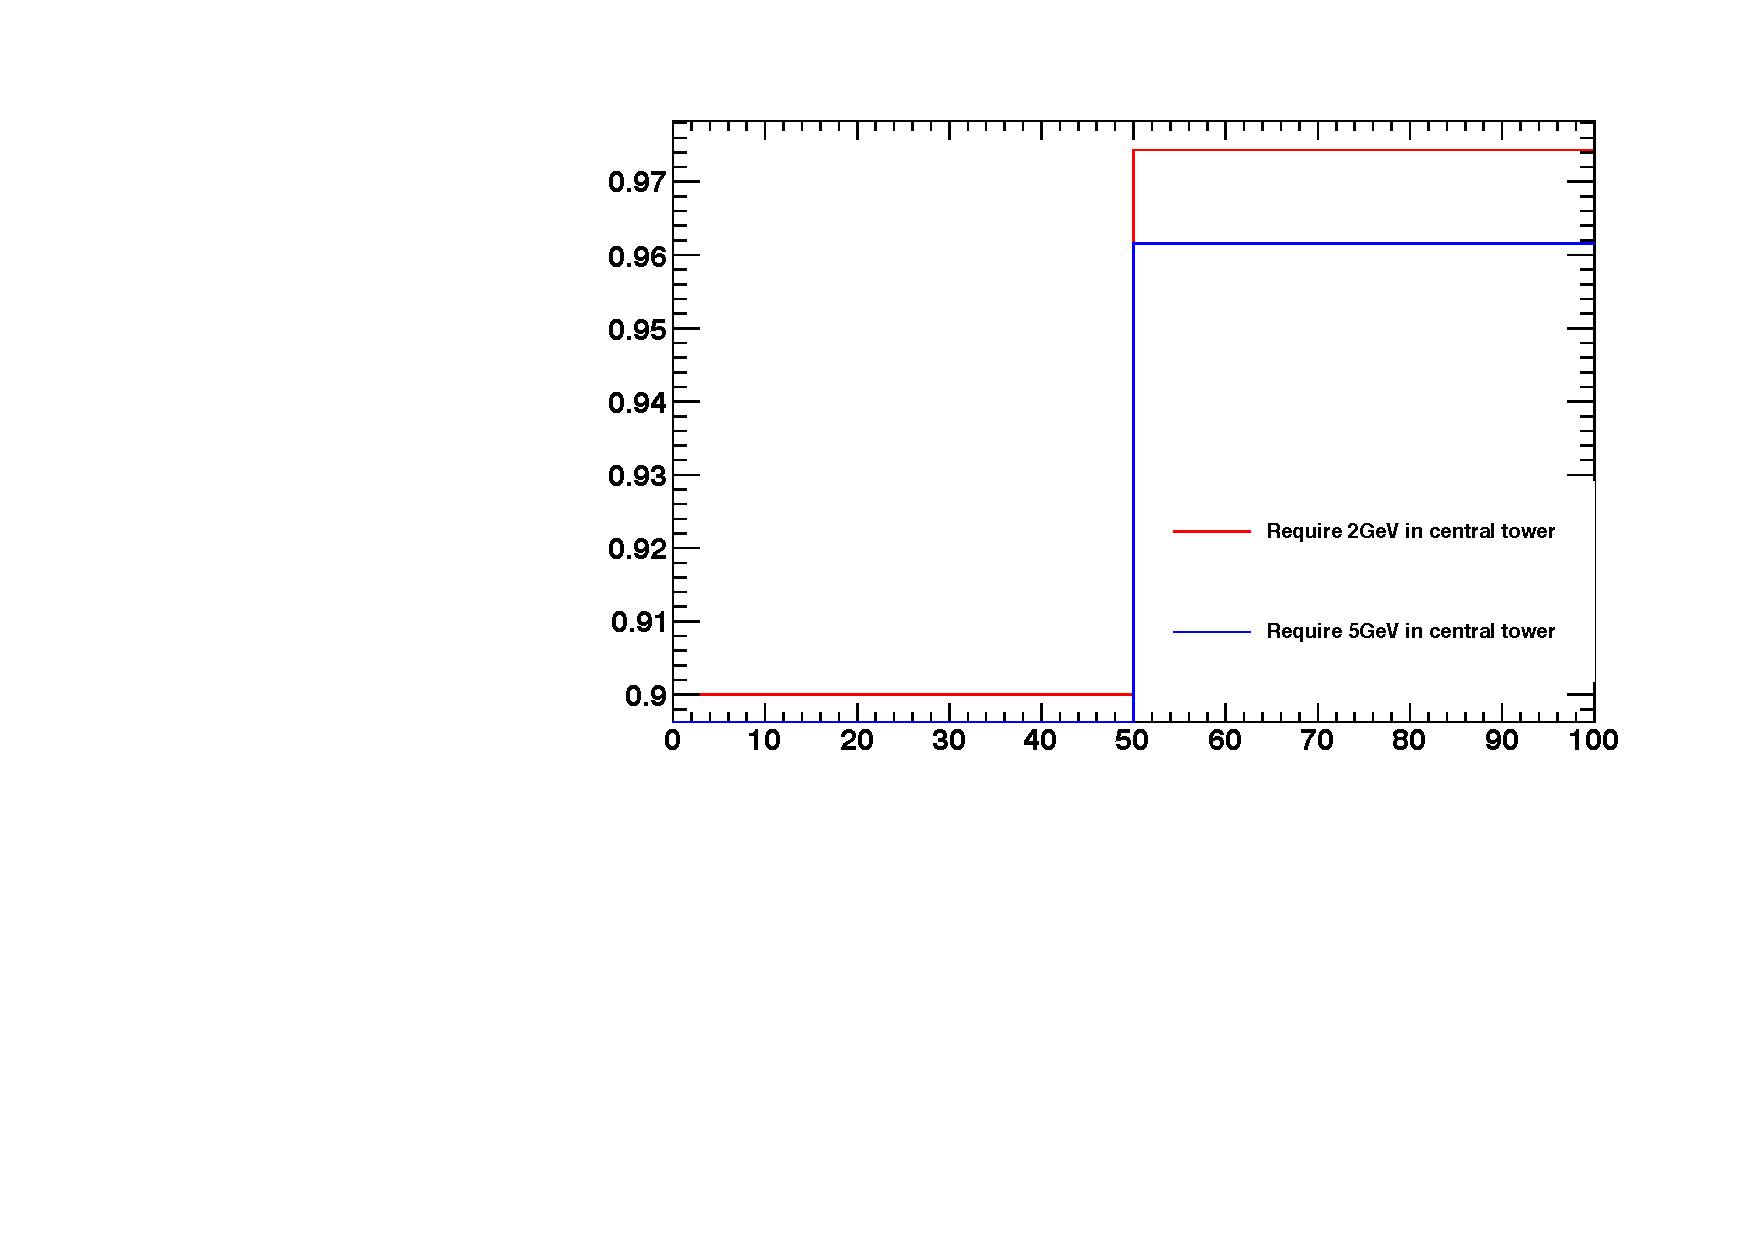
\includegraphics[width=0.46\textwidth]{figures/LoneTrigger/Cen_Tau_LowPU_RECO.pdf}
     }
     \newline
    \subfigure[]{
          \label{fig:quadJetLowPURECO}
          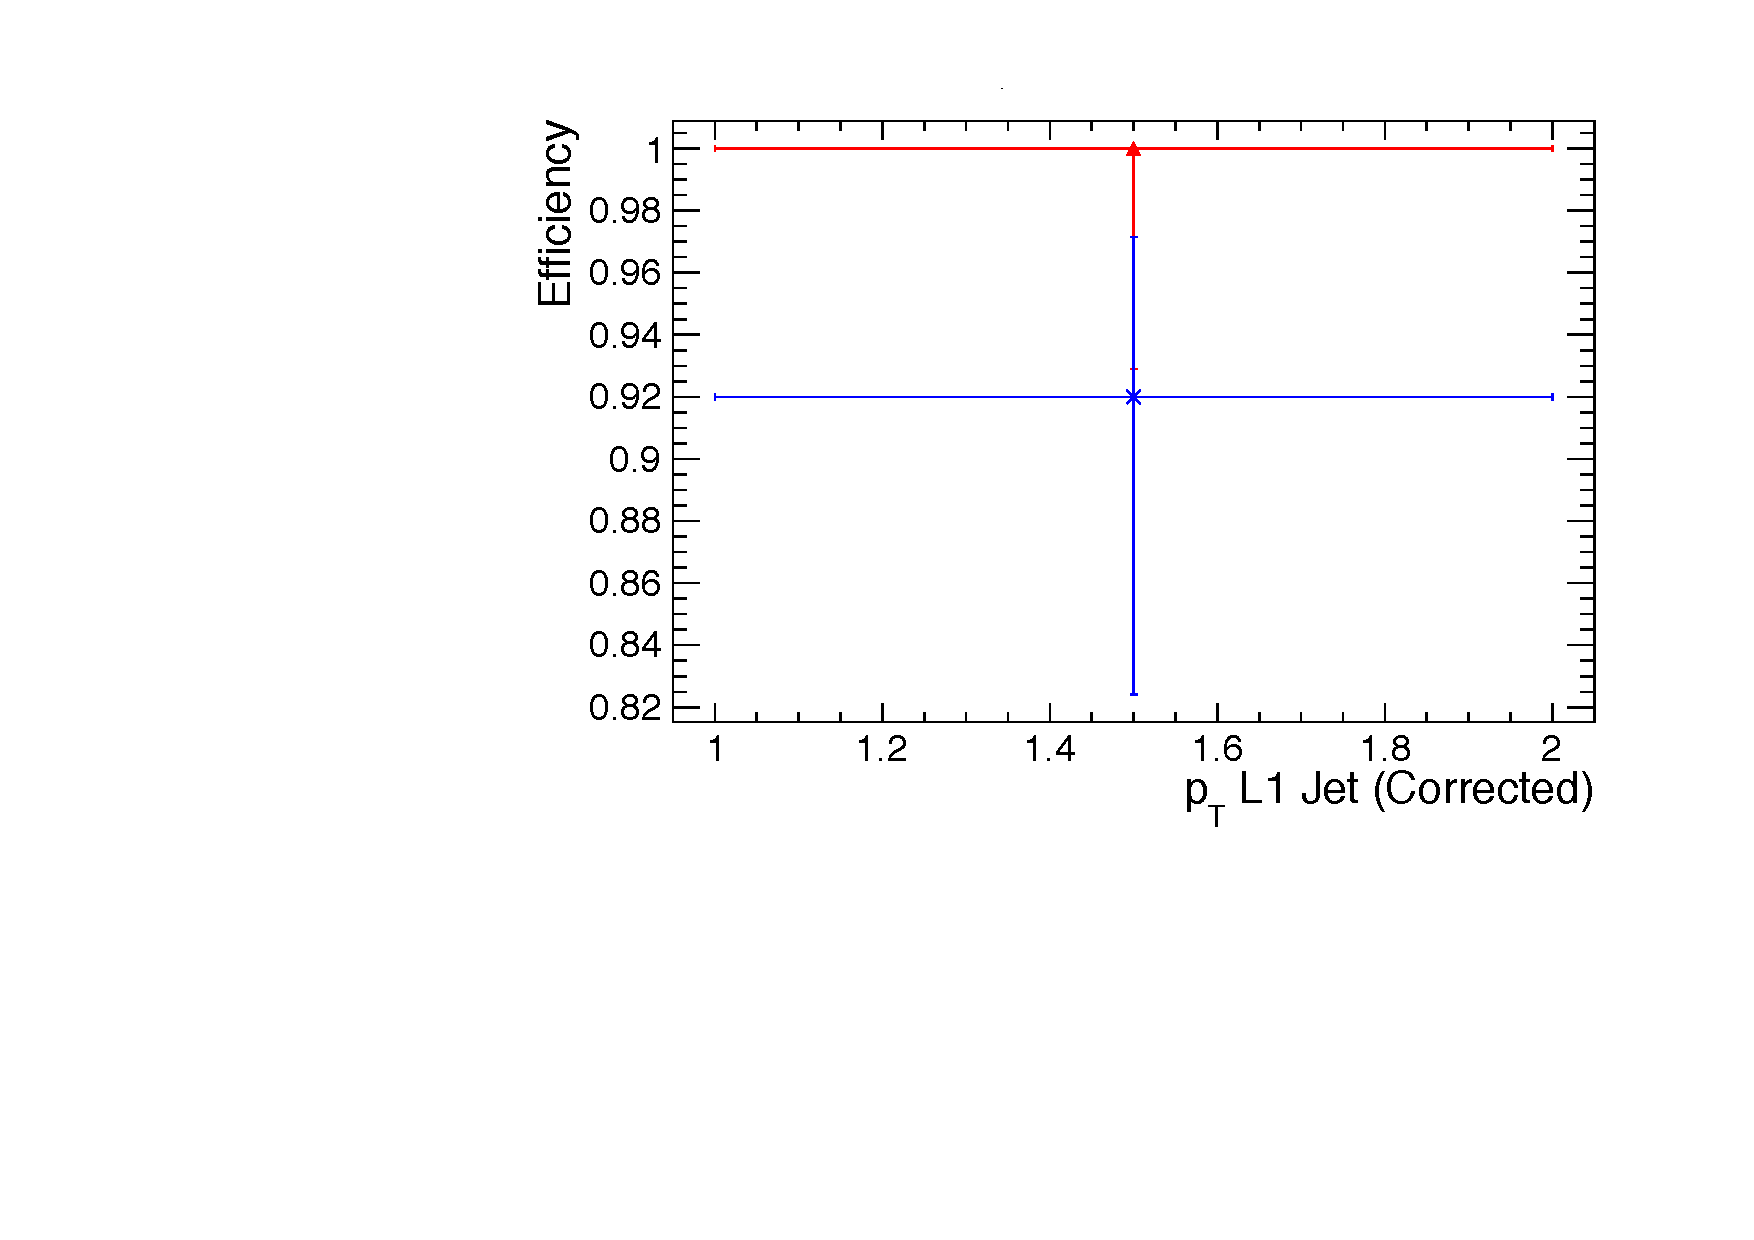
\includegraphics[width=0.46\textwidth]{figures/LoneTrigger/QuadJet_38Cen_LowPU_RECO.pdf}
     }
    \caption{Efficiency reductions for various \Lone algorithms when applying a 
    2 or 5 \GeV seed tower requirement, in low pile up 
    conditions. Figure (a) shows the efficiency reduction for \HT triggers at 
    low pile up in cut steps of 25 \GeV. Figure (b) 
    shows the efficiency reduction for jets with in $|\eta| <3.$ and $\pt > 
    50$\GeV. Figure (c) show the efficiency reduction for a quad jet trigger, 
    with jet $|\eta| <3.$ and $\pt > 38$\GeV.}
    
    \label{fig:lowpuratereduction}
\end{figure}



\paragraph{Efficiency of \HT Triggers} % (fold)
\label{par:Efficneicy of HT triggers}
Figure~\ref{fig:HTlowPURECO} shows the acceptance reduction after applying the 
two jet seed thresholds. The distribution is the cumulative number of events 
passing a cut of $L1 HT^{cut}$ in bins of 25 \GeV. Due to \HT being the scalar 
sum of the jet \PT's in the event the value of \Lone \HT is reduced as jets are 
removed from the calculation. To preserve efficiency the \Lone trigger 
threshold will have to be reduced. Comparing figures~\ref{fig:HTLowPU} and 
\ref{fig:HTlowPURECO}, if the trigger threshold is reduced to 75 \GeV an 
efficiency of $\geq 95\%$ can be maintained whilst reducing the trigger rate by 
$\approx 2\%$ when requiring a 2 \GeV seed threshold and reduced by $\approx 
3\%$ when requiring a 5 \GeV seed threshold. When comparing to the high pile up 
rate reduction in figure~\ref{fig:HTHighPU} it is shown that the trigger rate 
can be reduced by $\approx 20\%$ when requiring a 2 \GeV seed threshold and
reduced by $\geq 99\%$ when requiring a 5 \GeV seed threshold.
% subsection Efficneicy of \HT triggers (end)


\paragraph{Efficiency of Jet Triggers} % (fold)
\label{par:Efficiency of Jet Triggers}
Figure~\ref{fig:cenJetLowPURECO} shows the change in acceptance of jets in low 
pile up conditions when the two seed thresholds are required. The effect is on 
the order of a few percent for each of the thresholds. Requiring a 2 \GeV seed 
reduces the efficiency for jets above 50 \GeV by $\approx 2.5\%$, whilst 
requiring a 5\GeV seed reduces the efficiency of the same jets by $\approx 4\%$.
% subsection Efficiency of Jet Triggers (end)

\paragraph{Efficiency of MultiJet Triggers} % (fold)
\label{par:Efficiency of MultiJet Triggers}
Figure~\ref{fig:quadJetLowPURECO} shows that the effect of requiring a seed 
threshold of 2 \GeV has no effect on the efficiency of the quad jet 38 \GeV 
trigger and requiring a seed threshold of 5 \GeV reduces the efficiency of the 
quad jet 38 trigger by $8\%$. The change in rate is dramatic in high pile up 
conditions where for a 2 \GeV seed threshold the rate is reduced by 
$\approx 30\%$ and by $\approx 40\%$ when requiring a 5 \GeV seed.
However it is to be noted that the sample where this measurement has been made 
is of limited size, inferring a reasonably large statistical uncertainty. 
% subsection Efficiency of MultiJet Triggers (end)



% section Effects of requiring a jet seed on offline efficiency (end)

\subsection{Summary} % (fold)
\label{sec:Summary}
The effects of requiring a jet seed have been studied using the \Lone trigger 
emulator on high and low pile-up samples. The studies show that requiring a jet 
seed of 5\GeV greatly reduces the rate of the \HT and Multi Jet triggers in 
high pile up conditions, whilst not adversly effecting the data taking 
efficiency of these triggers.

\begin{figure}[ht]
  \centering
    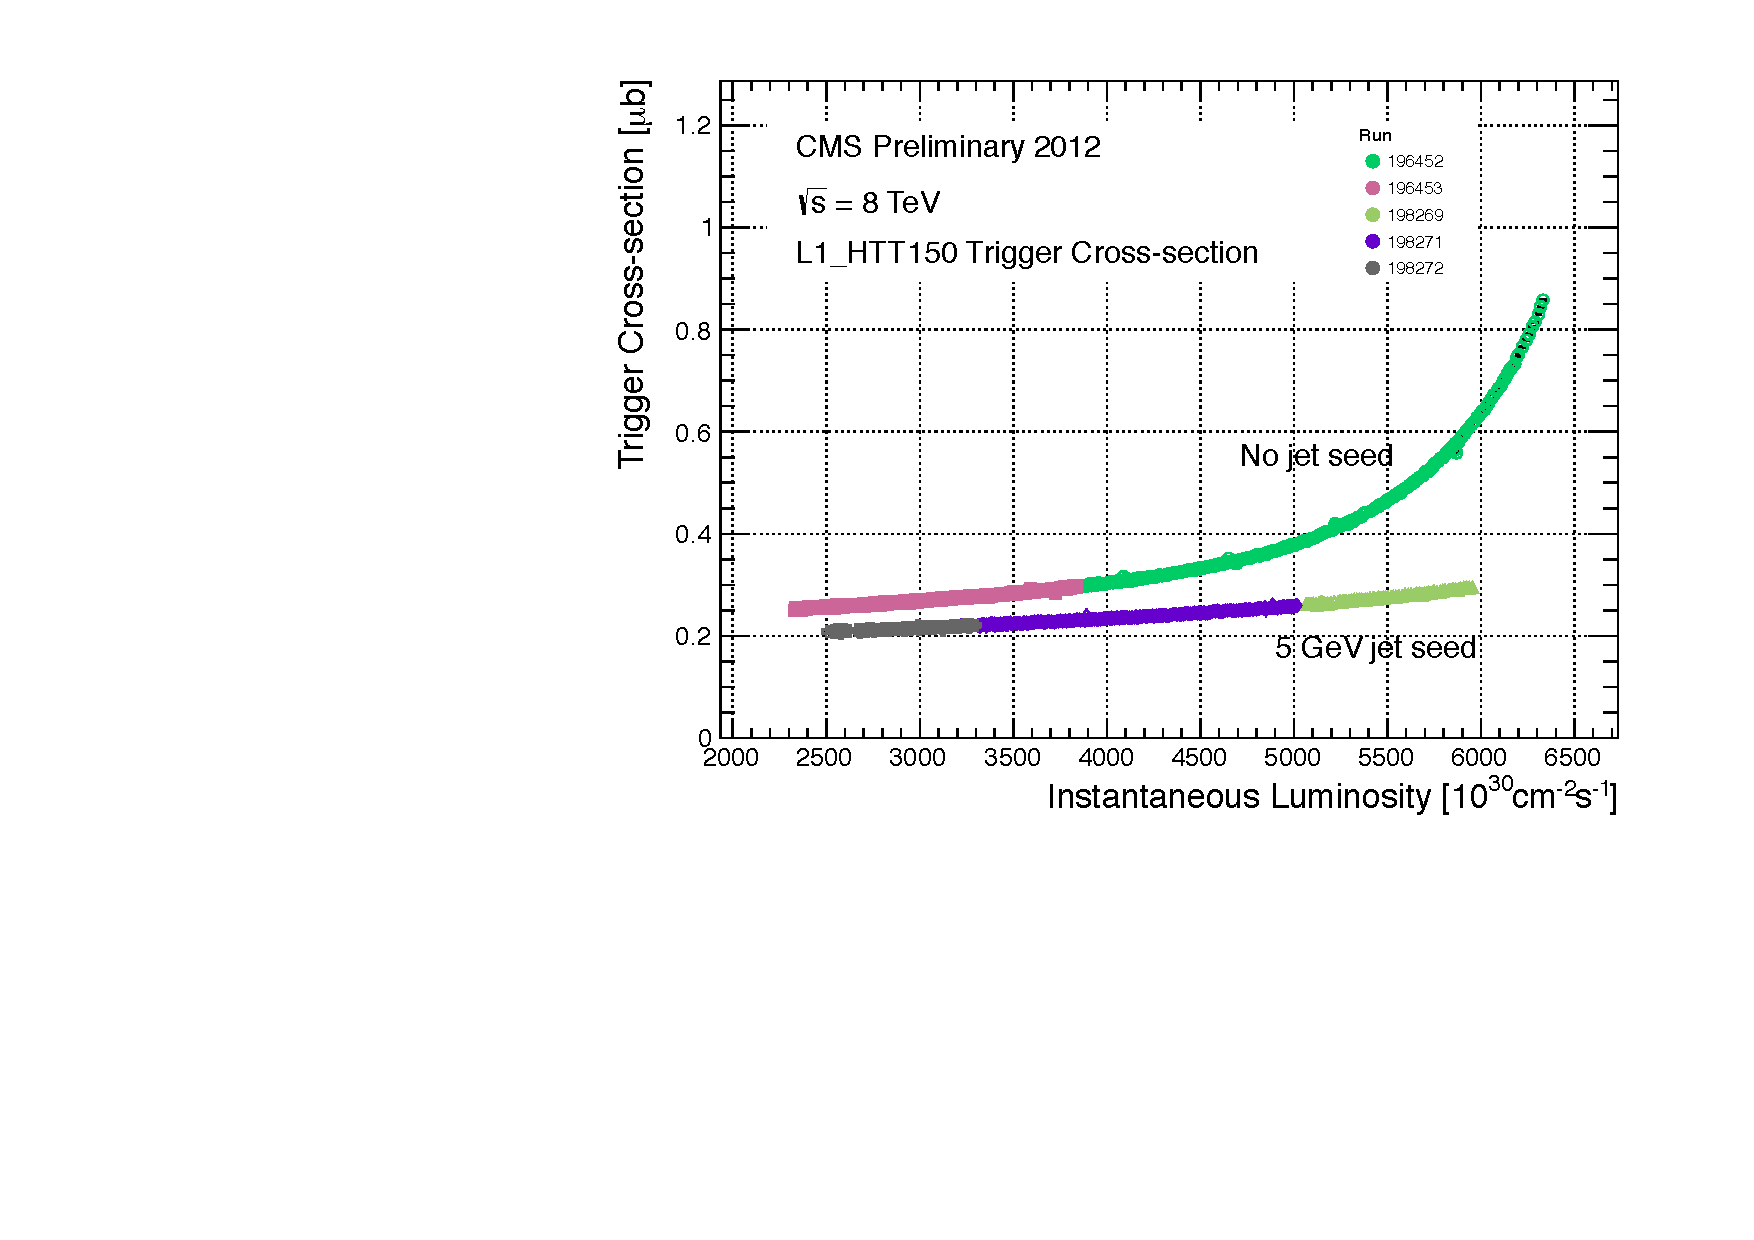
\includegraphics[width=0.75\textwidth]{figures/LoneTrigger/HTT150_pileup.pdf}
  \caption{Trigger cross section as a fucntion of number of pile up 
  interactions. Showing that applying a 5 \GeV jet seed threshold dramitically 
  reduces the quadratic dependance of cross section on the number of pile up 
  interactions}
  \label{fig:figures_HTT150_pileup}
\end{figure}

The cross section of L1$\_$HTT150 has been measured with and with out the 
addition of a jet seed threshold of 5 \GeV as shown in  
Figure~\ref{fig:figures_HTT150_pileup}. Idealy the trigger cross section would 
be independant of the instantanious luminosity and pile up, 
Figure~\ref{fig:figures_HTT150_pileup} shows that the addition of a 5 \GeV seed 
threshold reduces the dependance on instantanious luminosity of the trigger 
cross section.

% subsection lone_trigger_pile_up_mitigation (end)
% chapter level_one_trigger (end)
\input{chapters/Analysis}
\chapter{Conclusion} % (fold)
\label{cha:conclusion}

% chapter conclusion (end)
\end{mainmatter}
    



\begin{backmatter}
\bibliographystyle{plain}
\bibliography{thesis}

\end{backmatter}
\appendix
  \include{chapters/Appendix}
  \include{chapters/trigger_appendix}
  \include{chapters/backgroundestimation_appendix}
  \include{chapters/bkg_syst_appendix}
  \include{chapters/sig_syst_appendix}




\end{document}
